% !TEX Program = xelatex
% class
\documentclass[ngerman]{scrartcl}

% input preamble
\usepackage{iftex}

% text input and font
\ifluatex  % LuaLaTeX
    \usepackage{fontspec}
    % main font automatically: Latin Modern
    \IfFontExistsTF{Fira Code}{% true branch
        \setmonofont{Fira Code}[
            Contextuals=Alternate,  % Activate the calt feature
            StylisticSet={1,3,5,8}, % fontspec docs S. 46
            CharacterVariant={16}, % fontspec docs S. 37
            Numbers={SlashedZero} % fontspec docs S. 44
        ]}{% false branch
    }
\else  % pdfLaTeX
    \usepackage[utf8]{inputenc}  % input in UTF-8
    \usepackage[T1]{fontenc}  % output in T1 fonts (west European encoding)
    \usepackage{lmodern}  % Latin modern font for main text
    \IfFileExists{fira.sty}{% true branch
        \usepackage[mono]{fira}  % Fira (not Code!) font for monospaced text
    }{% false branch
    }
\fi

% text processing
\usepackage{babel}  % language package
\usepackage[intlimits]{mathtools}  % upgrade of amsmath (automatically loaded) - \int^_ like \limits^_
\usepackage{amssymb}  % upgrade of amsfonts (American Math Society)
\usepackage{amstext}  % \text command in math environments
\usepackage{letltxmacro}  % \let command for robust macros (new sqrt)
\usepackage{chemformula}  % typeset chemical formulas


% page geometry
\usepackage{scrlayer-scrpage}  % page formatting with KOMA options
\usepackage[paper=a4paper, hmargin=3cm, vmargin=2.5cm, includehead, includefoot]{geometry}  % horizontal: 3cm, vertical: 2.5cm strict with or without headers and footers
\usepackage{tabto}  % tab stops
\NumTabs{8}  % 8 equally spaced of \textwidth tab stops



% floats
\usepackage[hypcap=false, labelfont=bf]{caption, subcaption}  % caption editing - hypcap warning with hyperref
% counter prefixed with section number and therefore reset at each section:
\counterwithin{figure}{section}
\counterwithin{table}{section}
\usepackage{float}  % for [H] (forced here) specifier
\usepackage{tabularray}  % better tables
\usepackage{caption}  % better captions


% graphical input
\usepackage{graphicx}  % input JPEG, PNG, PDF, etc.
\usepackage{pdfpages}  % input PDF as whole pages
\usepackage{lastpage}  % reference to last page
\usepackage{import} % include files from other directories


% text
\usepackage[locale=DE, uncertainty-mode=separate]{siunitx}  % SI units, German formatting - \pm stays \pm instead of ..(.)
\let\sqty\qty  % physics overrides \qty of siunitx, therefore make it available as \sqty
\usepackage{physics}  % macros for easier typesetting of physical formulas
\usepackage{icomma}  % no space after commas instead of English points) in decimal values
\usepackage{enumitem}  % better enumerating with style options
\usepackage{nicefrac}  % inline-fractions in n/d-style
\usepackage{xcolor}  % custom colors
%TU-Graz colors
\definecolor{TUred}{HTML}{e4154b}
\definecolor{TUgray}{HTML}{bcbcbc}
\usepackage{listings, scrhack}  % code display; listings in combination with KOMA
\ifluatex
    \IfFontExistsTF{Fira Code}{%
        \usepackage[verbatim]{lstfiracode}  % Fira Code in listings
        \lstset{style=FiraCodeStyle}
    }{}
\fi
\usepackage{fancyvrb}  % Verbatim environment with better options (capital V!)


% literacy
\usepackage[sorting=none, giveninits=true]{biblatex}  % defaults: backend=Biber, style=numeric
% bibliography styles: https://www.overleaf.com/learn/latex/Biblatex_bibliography_styles
% citation styles: https://www.overleaf.com/learn/latex/Biblatex_citation_styles
\usepackage{csquotes}  % better quotation - should also be used in combination with package babel (warning)
\usepackage{xurl}  % breaks links - after BibLaTeX, but before hyperref!
\usepackage[hidelinks]{hyperref}  % produces most errors, last to load


% enumerate paragraphs and subparagraphs
% depths: https://www.overleaf.com/learn/latex/Sections_and_chapters
% -1 \part{part}
%  0 \chapter{chapter}
%  1 \section{section}
%  2 \subsection{subsection}
%  3 \subsubsection{subsubsection}
%  4 \paragraph{paragraph}
%  5 \subparagraph{subparagraph}
\setcounter{secnumdepth}{3}


% KOMA setups
% header and footer
\pagestyle{scrheadings}  % KOMA style
\clearpairofpagestyles  % reset
\setkomafont{pageheadfoot}{\normalfont}  % standard font in header and footer
\setlength{\headheight}{27.2pt}  % warning
\cfoot{\pagemark{} / \pageref*{LastPage}}  % center foot - *: ref but no hyperlink
% {}: empty statement
% \ : protected space
% \,: small space
\DeclareTOCStyleEntry[linefill=\TOCLineLeaderFill]{tocline}{section}  % sections in TableOfContents with dotted lines
% source: https://tex.stackexchange.com/a/651532
\KOMAoptions{parskip=half-}  % paragraphs with half a line height space instead of indentation, last line with no special treatment


% package setups

% rewrite names (babel overwrites German with standard English names, therefore at document beginn [after everything is loaded])
\AtBeginDocument{\renewcommand{\refname}{Literaturverzeichnis}}
% others:
% \contentsname
% \listtablename
% \listfigurename

% make title in bibliography upright
\DeclareFieldFormat{title}{#1}  % https://tex.stackexchange.com/a/311837
% make size of url in bibliography smaller
\renewcommand{\UrlFont}{\footnotesize\ttfamily}  % https://tex.stackexchange.com/a/151115, https://www.overleaf.com/learn/latex/Font_sizes%2C_families%2C_and_styles


% xcolor
\definecolor{code_keyword}{HTML}{A06E9D}
\definecolor{code_string}{HTML}{AD6E3E}
\definecolor{code_comment}{HTML}{6A9955}
% \definecolor{keyword_pink}{HTML}{c678dd}
% \definecolor{vscode_bg}{HTML}{282c34}
% \definecolor{vscode_var}{HTML}{e06c75}
% \definecolor{vscode_comment}{HTML}{7f848e}
% \definecolor{vscode_constant}{HTML}{d19a66}
% \definecolor{vscode_function}{HTML}{61afe3}
% \definecolor{background_grey}{HTML}{f8f8f8}
% \definecolor{code_basic}{HTML}{D4D4D4}
% \definecolor{code_background}{HTML}{1E1E1E}

% custom siunitx units
\DeclareSIUnit{\dig}{dig}  % digits for uncertainty of electronical measurement devices
\DeclareSIUnit{\px}{px}  % pixels
\sisetup{table-align-uncertainty=true}


% listings
\lstset{
    basicstyle=\ttfamily\footnotesize,%\color{code_basic},  % \footnotesize contains \selectfont implicitly
    %backgroundcolor=\color{code_background},
    commentstyle=\color{code_comment},
    keywordstyle=\bfseries\color{code_keyword},
    numberstyle=\tiny,
    stringstyle=\color{code_string},
    breakatwhitespace=false,
    breaklines=true,
    captionpos=b,
    keepspaces=true,
    numbers=left,
    numbersep=5pt,
    showspaces=false,
    showstringspaces=false,
    showtabs=false,
    tabsize=2
}


% new sqrt
% https://en.wikibooks.org/wiki/LaTeX/Mathematics
\makeatletter
\let\oldr@@t\r@@t
\def\r@@t#1#2{%
    \setbox0=\hbox{$\oldr@@t#1{#2\,}$}\dimen0=\ht0
    \advance\dimen0-0.2\ht0
    \setbox2=\hbox{\vrule height\ht0 depth -\dimen0}%
    {\box0\lower0.4pt\box2}}
\LetLtxMacro{\oldsqrt}{\sqrt}
\renewcommand{\sqrt}[2][\ ]{\oldsqrt[#1]{#2} }
\makeatother


% own commands
% \newcommand* can't contain multiple lines
% \newcommand can
\newcommand*{\mup}[1]{\ensuremath{\text{\textup{#1}}}}  % math mode upright normal font
\newcommand*{\inkgraphics}[3][\linewidth]{\def\svgwidth{#1}\import{#2}{#3}}
\newcommand{\todo}[1]{\textbf{\textcolor{TUred}{#1\\}}}


% custom tabularray environments

% imports and setups of tabularray: {
%     expl3,
%     xparse,
%     ninecolors
%     \hypersetup{pdfborder={0 0 0}}
% }

% additionally loaded libraries:
% diagbox
% varwidth
% booktabs
% counter

\UseTblrLibrary{amsmath}  % +array, +matrix, +bmatrix, +Bmatrix, +pmatrix, +vmatrix, +Vmatrix and +cases like tabularray with graphical options
\UseTblrLibrary{siunitx}  % siunitx suited for tabularray
\UseTblrLibrary{diagbox}  % table cells with diagonal lines, suited for tabularray
\UseTblrLibrary{varwidth}  % measure cell width
\UseTblrLibrary{booktabs}
\UseTblrLibrary{counter}


% custom tabularray environments:

% info:
% colcycle: https://github.com/lvjr/tabularray/issues/74
% guard: https://github.com/lvjr/tabularray/issues/175#event-6567229210

% guard S columns if latest feature ={guard} is not yet available
\newcommand*{\SiGuard}[1]{{#1}}

% standard environment
\SetTblrInner{
    hlines,
    vlines,
    columns={
            halign=c,
            valign=m,
        },
    measure=vbox,
}

% X columns
\NewTblrEnviron{tblrx}
\SetTblrInner[tblrx]{
    hlines,
    vlines,
    columns={
            halign=c,
            valign=m,
            co=1,  % coefficient of width for expendable columns (X columns)
        },
    width=\linewidth,
    vspan=minimal,
    measure=vbox,
}

% -X columns
\NewTblrEnviron{tblr-x}
\SetTblrInner[tblr-x]{
    hlines,
    vlines,
    columns={
            halign=c,
            valign=m,
            co=-1,  % shrinks X column down to natural width
        },
    width=\linewidth,
    vspan=minimal,
    measure=vbox,
}

% no hline and vline left and on top of first cell
\NewTblrEnviron{tblr_omit_first_cell}
\SetTblrInner[tblr_omit_first_cell]{
    hlines,
    vlines,
    columns={
            halign=c,
            valign=m,
        },
    hspan=even,
    vspan=minimal,
    %
    hline{1}={1}{white},  % first row, only first cell
    vline{1}={1}{white},
    measure=vbox,
}

% longtblr
\DefTblrTemplate{conthead-text}{default}{(Fortsetzung)}  % default: define and set at the same time
\DefTblrTemplate{contfoot-text}{default}{Fortsetzung auf nächster Seite}
\SetTblrStyle{caption-tag}{font=\bfseries}  % caption tag bold
\SetTblrInner[longtblr]{
    hlines,
    vlines,
    columns={
            halign=c,
            valign=m,
        },
    measure=vbox,
}

% longtblr - to adjust width of caption 
\DefTblrTemplate{firsthead}{default}{\addtocounter{table}{-1}\captionof{table}[\InsertTblrText{entry}]{\InsertTblrText{caption}}}
\DefTblrTemplate{middlehead,lasthead}{default}{\addtocounter{table}{-1}\captionof{table}[]{\InsertTblrText{caption}~(Fortsetzung)}}
%info ADD this to a local environment around the longtblr: \captionsetup{format=plain,labelfont=bf,font=small,  width=\linewidth}

% manual header
\ihead{Interferometrie}  % inner (left) head
\chead{\textsc{Wachmann} Elias (12004232)\\\textsc{Zach} Andreas (12004790)}  % center head
\ohead{10.03.2023}  % outer (right) head

\addbibresource{Interferometrie_2023.bib} %!TODO cite stuff



\begin{document}

%%%%Title Page %%%%
\begin{titlepage}
    \centering
    
\includegraphics[width=0.5\textwidth]{../../99_Misc/Logo_Uni_Graz.jpg}\par\vspace{0.8cm}
    {\scshape\LARGE Karl-Franzens-Universität Graz \par}
    {\scshape\LARGE Institut für Physik \par}
    \vspace{1cm}
    {\scshape\Large 23S PHY.L02UB Fortgeschrittenenpraktikum 2 LU
\par}
    678 Bachelorstudium Physik, UG2002/2021W\par
    \vspace{1.5cm}
    {\huge\bfseries II. Interferometrie\par}
    \vspace{2cm}
    \begin{table}[H]
        \centering
        \begin{tabular}{c c c}
           \Large Wachmann Elias & & \Large Zach Andreas \\
           \Large 12004232       & & \Large 12004790 \\
           \multicolumn{3}{c}{Gruppe 12}
        \end{tabular}
    \end{table}
    \vfill
    \Large Betreut von\par
    BSc. MSc. Thomas Georg \textsc{Boné}

    \vfill

% Bottom of the page
    {\large 10.03.2023\par}
\end{titlepage}
%%%%

\clearpage
\tableofcontents
\newpage

\section{Aufgabenstellung} %!TODO referenzieren
\label{sec:aufgabenstellung}
Der folgende Laborversuch gliedert sich in 4 Teilversuche welche sich abermals wie folgt in Unterversuche glieder:
\begin{itemize}
    \item Young'scher Doppelspalt
    \begin{itemize}
        \item Bestimmen des Beugungsmusters von vier Doppelspalten mit unterschiedlichen Spaltbreiten und Spaltabständen. 
        \item Daraus Berechnung der Wellenlänge des Lasers.
        \item Erklärung der Beugungsmuster durch Vergleich mit errechneten Mustern.
        \item Bestimmung der Beugungsmuster eines Liniengitters und vergleich mit errechneten Werten. 
        \item Bestimmung der Gitterkonstante
    \end{itemize}
    \item Wellenfront-Analyse / Shearing Interferometer
    \item Polarisation
    \begin{itemize}
        \item Verifizieren des Gesetzes von Malus
        \item Untersuchung des Einflusses des Durchlasswinkels eines weiteren Polarisators zwischen zwei gekreuzten Polarisatoren. 
    \end{itemize}
    \item Michelson Interferometer
    \begin{itemize}
        \item Justieren und generieren von konzentrischen Interfernzmustern. 
        \item Bestimmung der Wellenlänge des Lasers durch Weglängenänderung. 
        \item Untersuchung des absoluten Weglängenunterschieds in den beiden Interferometerarmen, sowie Auflösung und Stabilität des Interferometers. 
        \item Untersuchung der Rolle der Polarisation auf die Interfenzfähigkeit des Laserlichts. 
    \end{itemize}
\end{itemize}


\section{Grundlagen} %!TODO referenzieren
\label{sec:grundlagen}
\subsection{Young'scher Doppelspalt}
\label{sec:grundlagen_youngscher_doppelspalt}
Bescheint man mit einer Lichtquelle zwei eng beieinander liegende Spalte mit dem Abstand $d$ in einem ansonsten undurchsichtigen Schirm, so wirkt die Spalte als kohärente Lichtquellen (Anmerkung: Dies ist evident für einen kohärente Lichtquelle, gilt für eine thermische Lichtquelle aber nur unter bestimmten Bedingungen, jenen der räumlichen Kohärenz). Die Wellen aus den Spalten überlagern sich in Abhängigkeit vom Beobachtungswinkel konstruktiv oder destruktiv, was auf einen Schirm projiziert eine Abfolge an Intensitätsmaxima und -minima ergibt. Unter der Bedingung, dass der Abstand zwischen Doppelspalt und Beobachtungsebene viel größer als der Spaltabstand $d$ ist, ergibt sich der optische Gangunterschied in die durch den Winkel $\phi$ definierte Richtung als ($\lambda$ Wellenlänge)

\begin{equation}
    \Delta = \frac{2 \pi d}{\lambda} \sin \phi
\end{equation}
Mit der Näherung $\sin \phi \approx \nicefrac{x}{z}$ (erfüllt für große Abstände $z$ zwischen Doppelspalt und Schirm) ergibt sich ein Streifenmuster mit der Periode $x$ der Form
\begin{equation}
    I(x)_{\text{Interferenz}} = I_0(1+ \cos \frac{2 \pi x d}{\lambda z})
\end{equation}
Dafür wurde die endliche Breite des Spalts vernachlässigt bzw. ein unendlich schmaler Spalt angenommen. Tatsächlich überlagert sich dem Interferenzmuster das Beugungsmuster des Einzelspalts, das i.A. symmetrisch mit zu größeren Winkeln hin abnehmender Intensität ist. Ein einzelner rechteckiger Spalt der Breite $D$ führt zu einem Beugungsmuster der Form
\begin{equation}
    I(x)_{\text{Beugung}} = I_0 \frac{\sin^2 \frac{\pi D x}{\lambda z}}{\left(\frac{\pi D x}{\lambda z}\right)^2}
\end{equation}
Das Beugungsmuster des Doppelspalts ergibt sich multiplikativ als $I(x) = I(x)_{\text{Interferenz}} \cdot I(x)_{\text{Beugung}}$.
\subsection{Shearing-Interferometer / Wellenfront-Analyse}
\label{sec:grundlagen_shearing_interferometer}
Das Erscheinungsbild von optischen Interferenzmustern ist sowohl durch die Natur der Lichtwelle als auch der optischen Grenzflächen bestimmt, man denke an die färbigen Interferenzen auf Seifenblasen. Entsprechend ist es möglich, aus der Beobachtung von Interferenzen an Grenzflächen bekannter Geometrie auf die Eigenschaften der Lichtwelle zu schließen.

%? Evtl. Bilder
Beim Shearing-Interferometer handelt es sich um ein simples Interferometer, mit dem bestimmt werden kann, ob ein Lichtstrahl kollimiert, konvergent oder divergent ist. Dazu trifft das Licht unter $45°$ auf eine Glasplatte, welche keilförmig ausgeführt ist. Durch die Reflexion an der vorderen und hinteren Fläche der Glasplatte entstehen zwei reflektierte Strahlen (Abb. 5a), in deren Überlappungsbereich Interferenz auftritt (Abb. 5b). Durch die keilförmige Geometrie führt dies für einen kollimierten Strahl zu einem zur Einfallsebene des Lichts parallelen Streifenmuster (Abb. 5b). Ein konvergierender bzw. divergierender Strahl führt dagegen nach Abb. 5b zu einem gedrehten Streifenmuster. Aus dem lateralen Versatz der beiden reflektierten Strahlen $l$, dem Streifenabstand $s$ und dem (bezogen auf die Senkrechte) Winkel der Interferenzstreifen $\Theta$ (siehe Abb. 5b) lässt sich der Radius $r$ der Wellenfront mit $r = \nicefrac{ls}{\lambda \sin \Theta}$ berechnen.
%ggf hier ein Bild
\subsection{Polarisation}
\label{sec:grundlagen_polarisation}
Für den Fall linearer Polarisation gilt für die transmittierte Intensität durch einen Polarisator mit der Durchlassrichtung entlang der durch den Winkel Null definierten Richtung das Gesetz von Malus.
\begin{equation}
    I(\alpha) = I_0 \cos^2 \alpha
\end{equation}
Die nicht transmittierte Intensität wird je nach Art des Polarisators absorbiert oder reflektiert. Die Polarisation ist entscheidend für die Interferenzfähigkeit von Licht, es gelten die vier Gesetze nach Fresnel und Arago \textbf{(siehe dazu auch einen entsprechenden Versuch mit dem Michelson-Interferometer)}.
\begin{itemize}
    \item In dieselbe Richtung linear polarisierte Lichtstrahlen interferieren (wie nicht polarisiertes Licht).11
    \item Zueinander senkrecht linear polarisierte Lichtstrahlen interferieren nicht (mit den folgenden Einschränkungen).
    \item Zueinander senkrecht linear polarisierte Lichtstrahlen interferieren, wenn sie ursprünglich dieselbe Polarisationsebene besaßen und wieder in diese zurückgeführt werden.
    \item  Zueinander senkrecht linear polarisierte Lichtstrahlen interferieren nicht, wenn sie in dieselbe Polarisationsebene zurückgeführt werden, diese aber nicht ursprünglich besaßen.
\end{itemize}

\subsection{Michelson-Interferometer} %? evtl. noch ein Bild
\label{sec:grundlagen_michelson_interferometer}
Der prinzipielle Strahlengang eines Michelson-Interferometers ist in Abb. 8 dargestellt. Ein Lichtstrahl aus einer (Laser-)Quelle (1) wird an einem Strahlteiler (2) aufgeteilt. Der Strahlteiler ist ein dünnes Glasplättchen mit einer teilreflektierenden Schicht auf einer Fläche. Die beiden resultierenden Lichtstrahlen werden an zwei Spiegeln reflektiert und am Strahlteiler wieder vereint. Die Lichtstrahlen im Detektorarm treffen auf den Schirm (4), wo sie sich in Abhängigkeit vom Unterschied der Weglängen s1 und s2 überlagern. Für ebene Wellen der Form
\begin{equation}
    E(x,t) = E_0 \exp{\omega t - k x}
\end{equation}
ist die Lichtintensität am Beobachtungsschirm gegeben durch
\begin{equation}
    I = \nicefrac{1}{4} c \epsilon_0 E_0^2 (1+\cos{\Delta \phi})
\end{equation}
wobei $\Delta \phi$ die Phasendifferenz bezeichnet, die mit dem Unterschied der Weglängen $\Delta s = \left| s_1  - s_2 \right|$ nach $\Delta \phi = (\nicefrac{2 \pi}{\lambda})\Delta s$ zusammenhängt. 

Es stellt sich die Frage, wo bei destruktiver Interferenz im Detektorarm die Energie der Lichtwellen bleibt. Tatsächlich hat das Interferometer ja zwei „Ausgänge“, wobei einer eben zum Beobachtungs-schirm, der zweite zurück zum Laser führt. Tatsächlich beobachtet man in zweiterem konstruktive Interferenz, wenn am Schirm destruktive Interferenz (also keine Lichtintensität) zu beobachten ist.

Das am Schirm beobachtete Interferenzmuster reagiert empfindlich auf kleine Änderungen in der Richtung des einfallenden Laserstrahls und in der Ausrichtung der Spiegel. Gleichzeitig sind diese Änderungen durch den nur wenige mm durchmessenden Strahl schwer zu beobachten. Deshalb wird der Strahl durch eine Linse aufgeweitet, was zwischen Laser und Strahlteiler oder zwischen Strahlteiler und Schirm geschehen kann. Ersteres führt zu einem konzentrischen Interferenzmuster, zweiteres zu parallelen Interferenzstreifen. Wie in Abb. 9a skizziert, können divergierende Strahlen auf (bei Vorliegen eines Weglängenunterschieds $\Delta s$ zwischen den beiden Interferometerarmen) auf zwei virtuelle Lichtquellen A und B zurückgeführt werden, wodurch sich das Auftreten eines konzentrischen Interferenzmusters erklärt. Gleichzeitig kann dieses genutzt werden, um die Interferometerarme auf die gleiche Länge einzustellen (im Prinzip auf einen Bruchteil der Wellenlänge), da sich dabei nach Abb. 9b die Größe des zentralen Interferenz“spots“ maximiert. Alternativ könnte dazu eine breitbandige Lichtquelle mit geringer Kohärenzlänge verwendet werde, wobei die Kohärenzlänge durch die Verwendung von Bandpassfiltern erhöht werden kann.

\section{Geräteliste}
\label{sec:geraeteliste}

Für den praktischen Aufbau und die Messungen der geforderten Größen wurden die in \autoref{tab:geraeteliste} aufgelisteten Geräte und Hilfsmittel verwendet.

\begin{table}[H]
    \centering
    \begin{samepage}
        \caption[Geräteliste]{Verwendete Geräte und wichtige Materialien}
        \label{tab:geraeteliste}
        \begin{tblrx}{cells={font=\footnotesize}}
            Gerät & Hersteller & Modell & Messsbereich / Unsicherheit & Inventar-Nr. \\
            Laser & Thorlabs & CPS532 &$\lambda = 532$&22442-S01\\
            diverse Spiegel & Thorlabs & KM100 &- &- \\
            Graufilter & Thorlabs & NX1N/M &- &- \\
            Doppelspalte & Phywe & 0852300 &- &- \\
            Gitter & Phywe & 0852400 &- &- \\
            Optischer Tisch& - & - &- &- \\ 
            diverse Halterungen & Thorlabs & - &- &- \\
            Sammellinse & Thorlabs & FMP1/M &f = $40$ mm &- \\
            Zerstreuungslinse & Thorlabs & FMP1/M &f = $-16$ mm &- \\
            Shearing-Interferometer & Thorlabs & nicht vorhanden &- &- \\
            Lichtintensitätsmesser & Sauter & SO 200k & $\Delta I = (\pm 3\% \text{rdg} \pm 0.5\% \text{fs}) \cdot I$ &51152203 \\
            Polarisationsfolie & Nitto denko & - &- &- \\
            Maßband& Schuller Eh klar& Power Tape $3$ m& Klasse 2 &- \\
            Michelson Interferometer & - & - &- &- \\
            Rohr & - & - &- &- \\
            diverse Abbildungsschirme & Wand, Papier, Tür, etc. & - &- &- \\
            Mobiltelefon & OnePlus & $8$-Pro &- &- \\

        \end{tblrx}
    \end{samepage}
\end{table}
Die verwendeten Doppelspalte haben folgende Abmessungen in \autoref{tab:doppelspalt_abmessungen}:
\textbf{TABELLE FEHLT NOCH!}
% \begin{table}[H] %! Irgendeinen schmarn mags da ned. will jetzt grad ned debuggen. 
%     \centering
%     \begin{samepage}
%         \caption[Doppelspaltmaße]{Verwendete Doppelspalte. Mit der jeweiligen Nummer $i$, der Spaltbreite $D$ in $\unit{\milli\meter}$ und dem Spaltabstand $d$ in $\unit{\milli\meter}$}
%         \label{tab:doppelspalt_abmessungen}
%         \begin{tblr}{colspec = {Q S[table-format=1.1]S[table-format=1.2]},row{1}={guard}}
%             $i$ / 1& $D$ / \si{\milli\meter} & $d$ / \si{\milli\meter} \\
%             1 & 0.2 & 0.25 \\
%             2 & 0.1 & 0.25 \\
%             3 & 0.1 & 0.50 \\
%             4 & 0.1 & 1.00 \\
%         \end{tblr}
%     \end{samepage}
% \end{table}

\textbf{Anmerkung zu den Unsicherheiten:}\\
Zur Unsicherheitsangabe werden die jeweiligen Unsicherheitsmaße der Geräte, welche aus den Datenblättern (sofern vorhanden) entnommen werden, verwendet. Für die analogen Messgeräte wird eine kombinierte Ablese- und Mess-Unsicherheit von $\pm$ 1 Skalenstrich verwendet.

Alle Teilversuche wurden bei einer Umgebungstemperatur von \SI{24(1)}{\celsius} einem Luftdruck von \SI{1000(10)}{\hecto\pascal} und einer relativen Luftfeuchtigkeit von \SI{33(1)}{\percent} durchgeführt.


\section{Versuchsaufbau}
\label{sec:aufbau}
\subsection{Young'scher Doppelspalt}
\label{sec:aufbau_doppelspalte}
Für den Aufbau zum Versuch Young'scher Doppelspalt wird der Laser mittels zwei Spiegel auf das Plättchen mit den 4 verschiedenen (siehe \autoref{tab:doppelspalt_abmessungen}) Doppelspalten gelenkt. Der Abstand vom Doppelspalt wird zu \SI{2520(5)}{\milli\meter} - wobei hier noch zur vom Maßband gegebenen Unsicherheit von \SI{1.1}{\milli\meter} eine weitere Unsicherheit durch das Messen in der Luft hinzukommt - bestimmt. Der Aufbau in \autoref{fig:aufbau_doppelspalt} zeigt den optischen Tisch, der Schirm ist rechts im oben angeführten Abstand an der Wand befestigt. 
\begin{figure}[H]
    \centering
    \begin{samepage}
        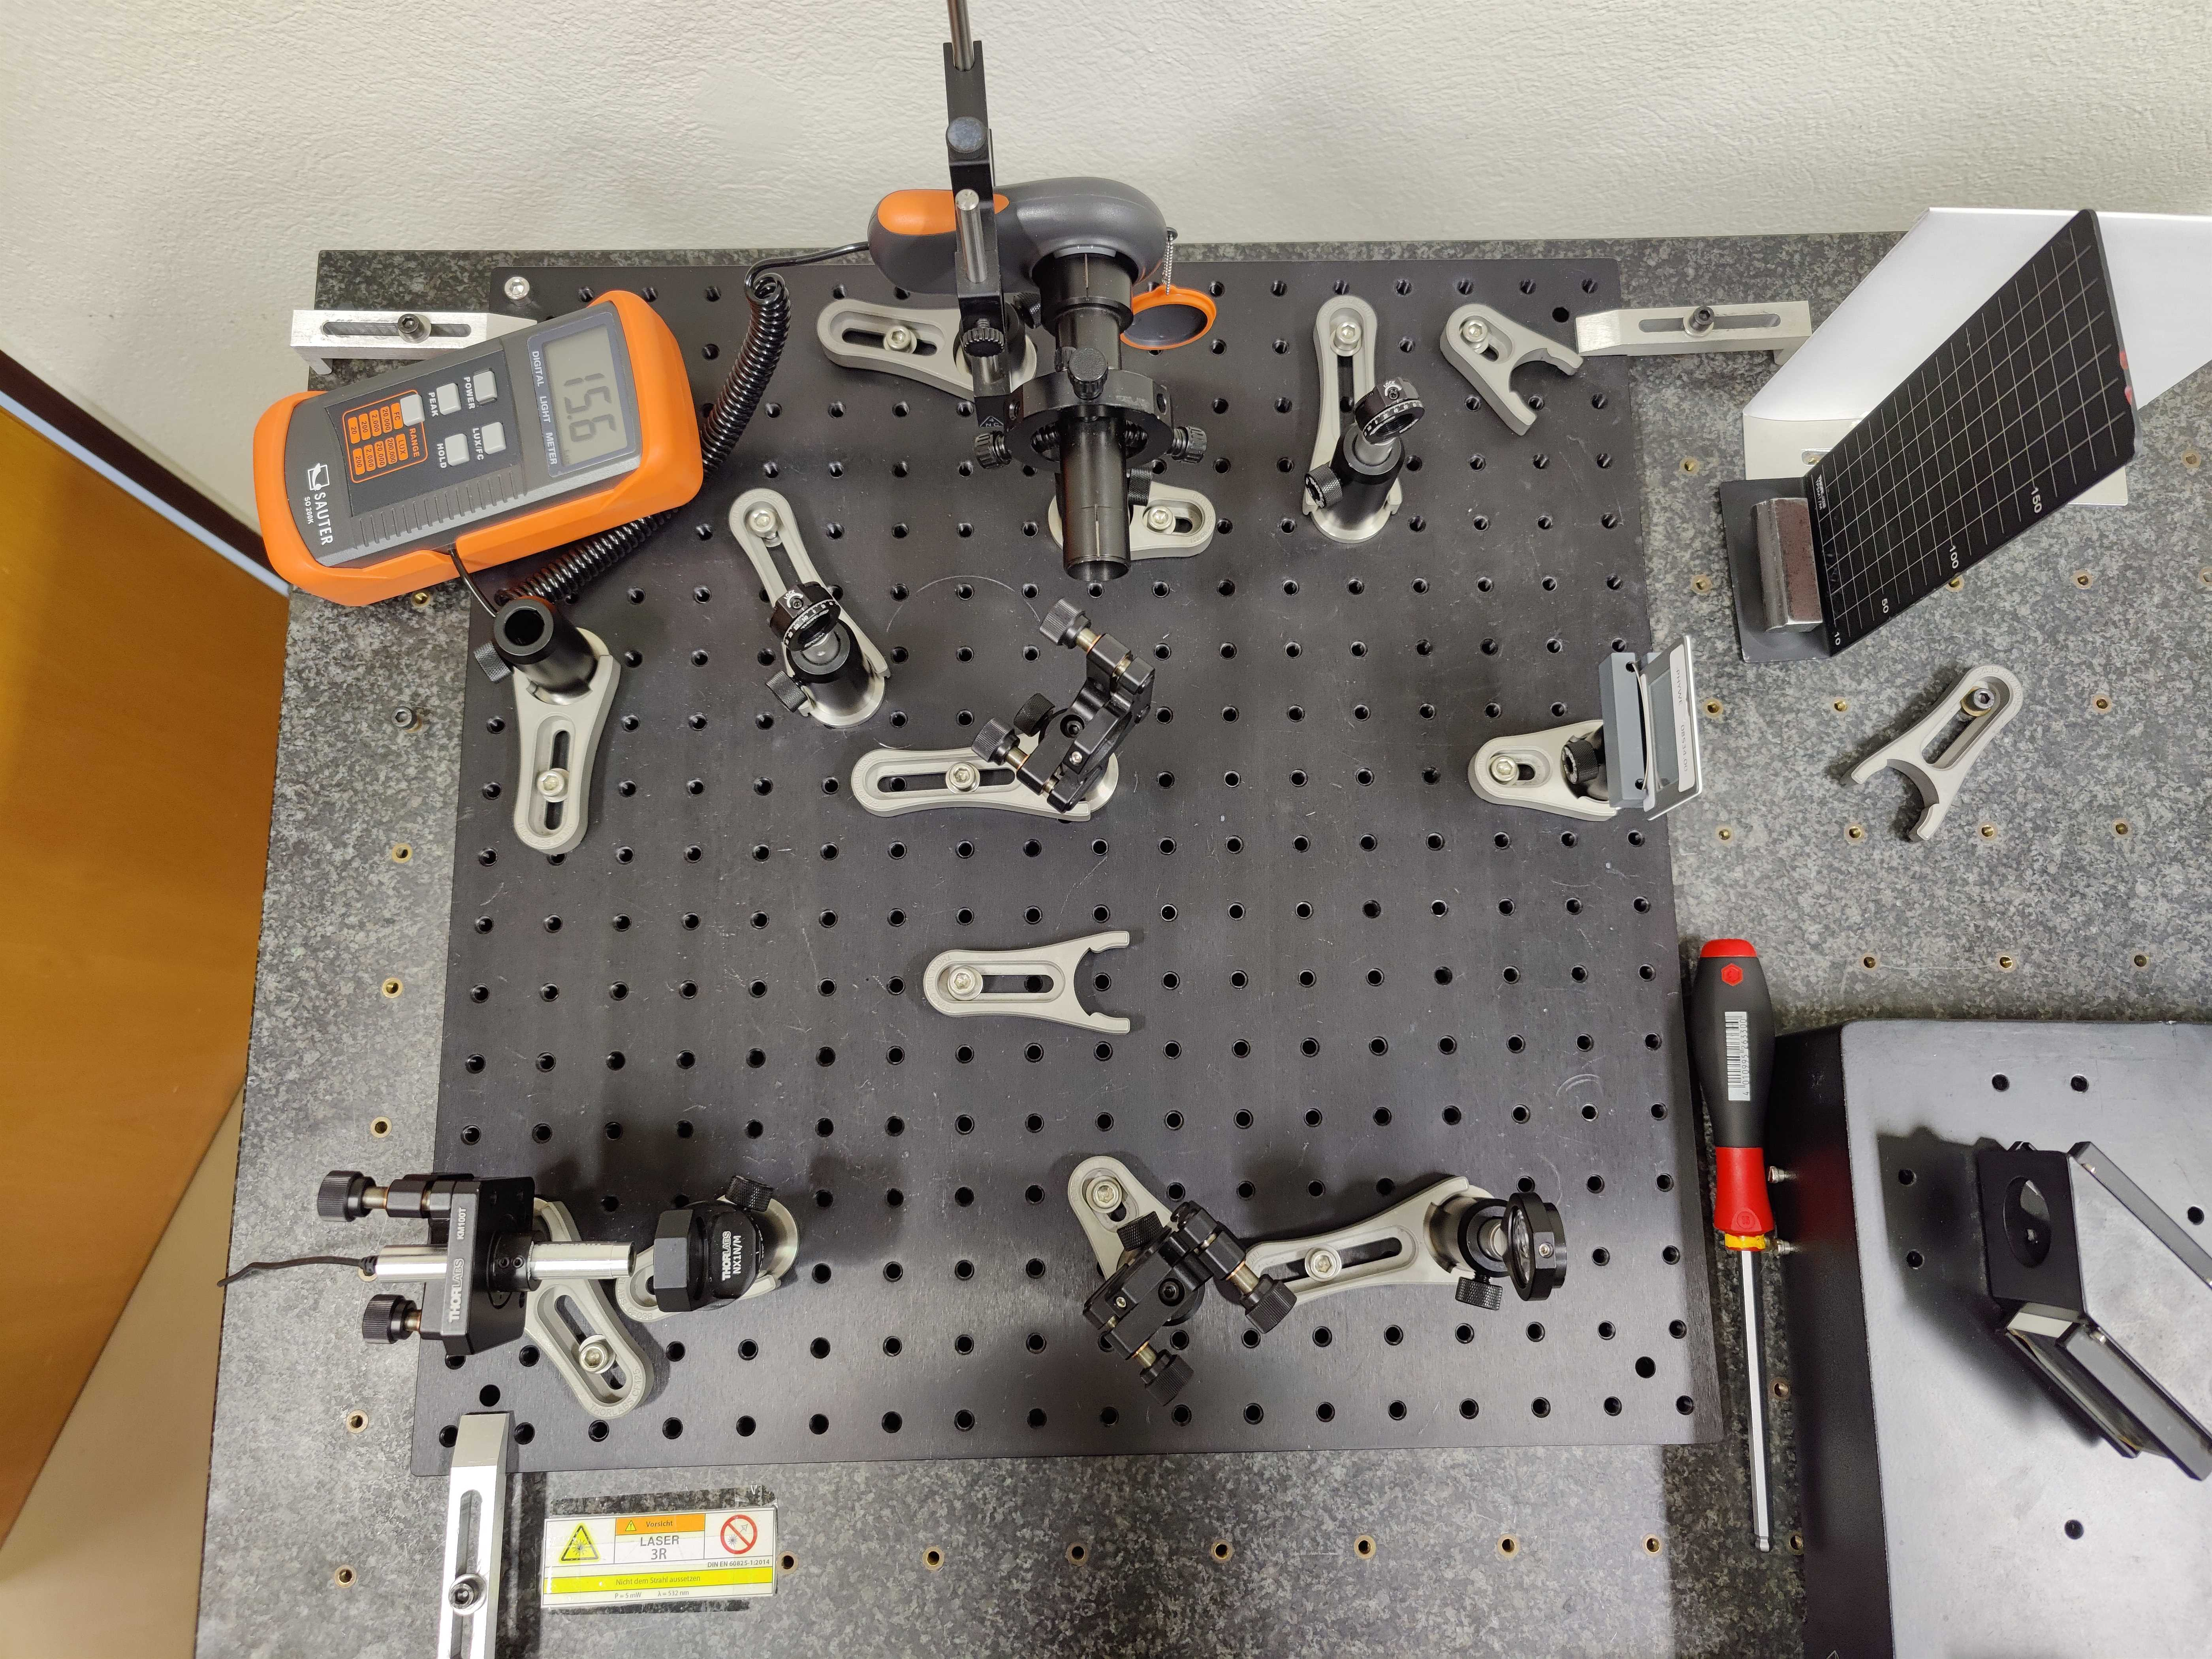
\includegraphics[width=0.7\linewidth]{fig/aufbau_doppelspalt.jpg}
        \caption{Aufbau young'scher Doppelspalt}
        \label{fig:aufbau_doppelspalt}
    \end{samepage}
\end{figure}
\subsection{Shearing Interferometer}
\label{sec:aufbau_shearing}
Der Aufbau des Shearing Interferometers ist in \autoref{fig:aufbau_shearing} gegeben. Dabei wird der untere Spiegel aus dem vorhergehenden Versuch wieder verwendet und der Laserstrahl auf die Frontalebene - welche um \SI{45}{\degree} zur Tischebene geneigt ist - gelenkt. 
\begin{figure}[H]
    \centering
    \begin{samepage}
        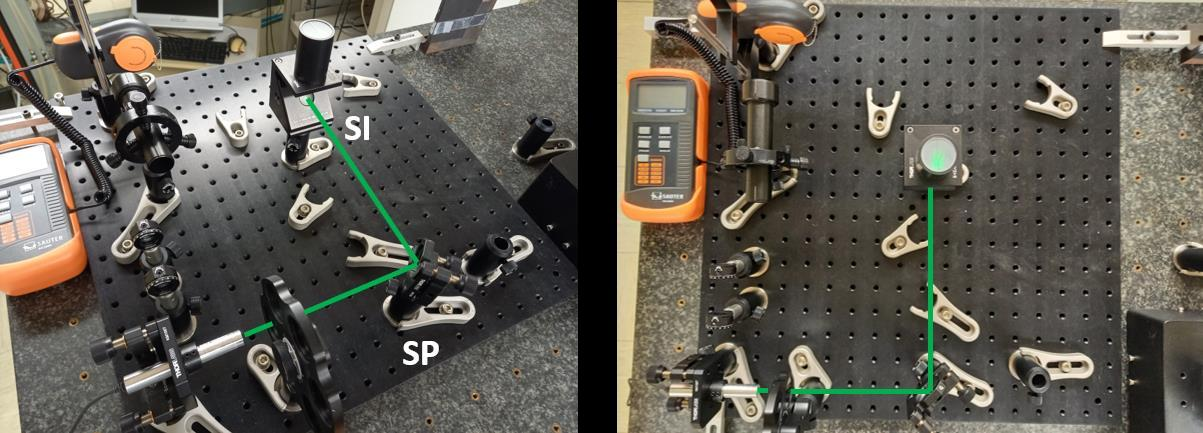
\includegraphics[width=0.9\linewidth]{fig/shearing.jpg}
        \caption{Aufbau Shearing Interferometer \textbf{CITE THIS!!!!}}
        \label{fig:aufbau_shearing}
    \end{samepage}
\end{figure}
\textbf{Anmerkung zum Versuch:} Da sich das Shearing Interferometer leider zum Zeitpunkt der Übung in Reparatur befand, wird der Versuch im folgenden hyptotethisch abgehandelt.  
\subsection{Polarisation}
\label{sec:aufbau_polarisation}
Anstelle des Shearing Interferometers werden jetzt zwei Polarisationsfilter in den Laserstrahl eingebracht. Nach dem zweitem Filter trifft der Laser auf einen Lichtintensitätsmesser welcher, wie in \autoref{fig:aufbau_polarisation} ersichtlich, durch ein Rohr von sonstigen Lichteinflüssen abgeschirmt wird.
\begin{figure}[H]
    \centering
    \begin{samepage}
        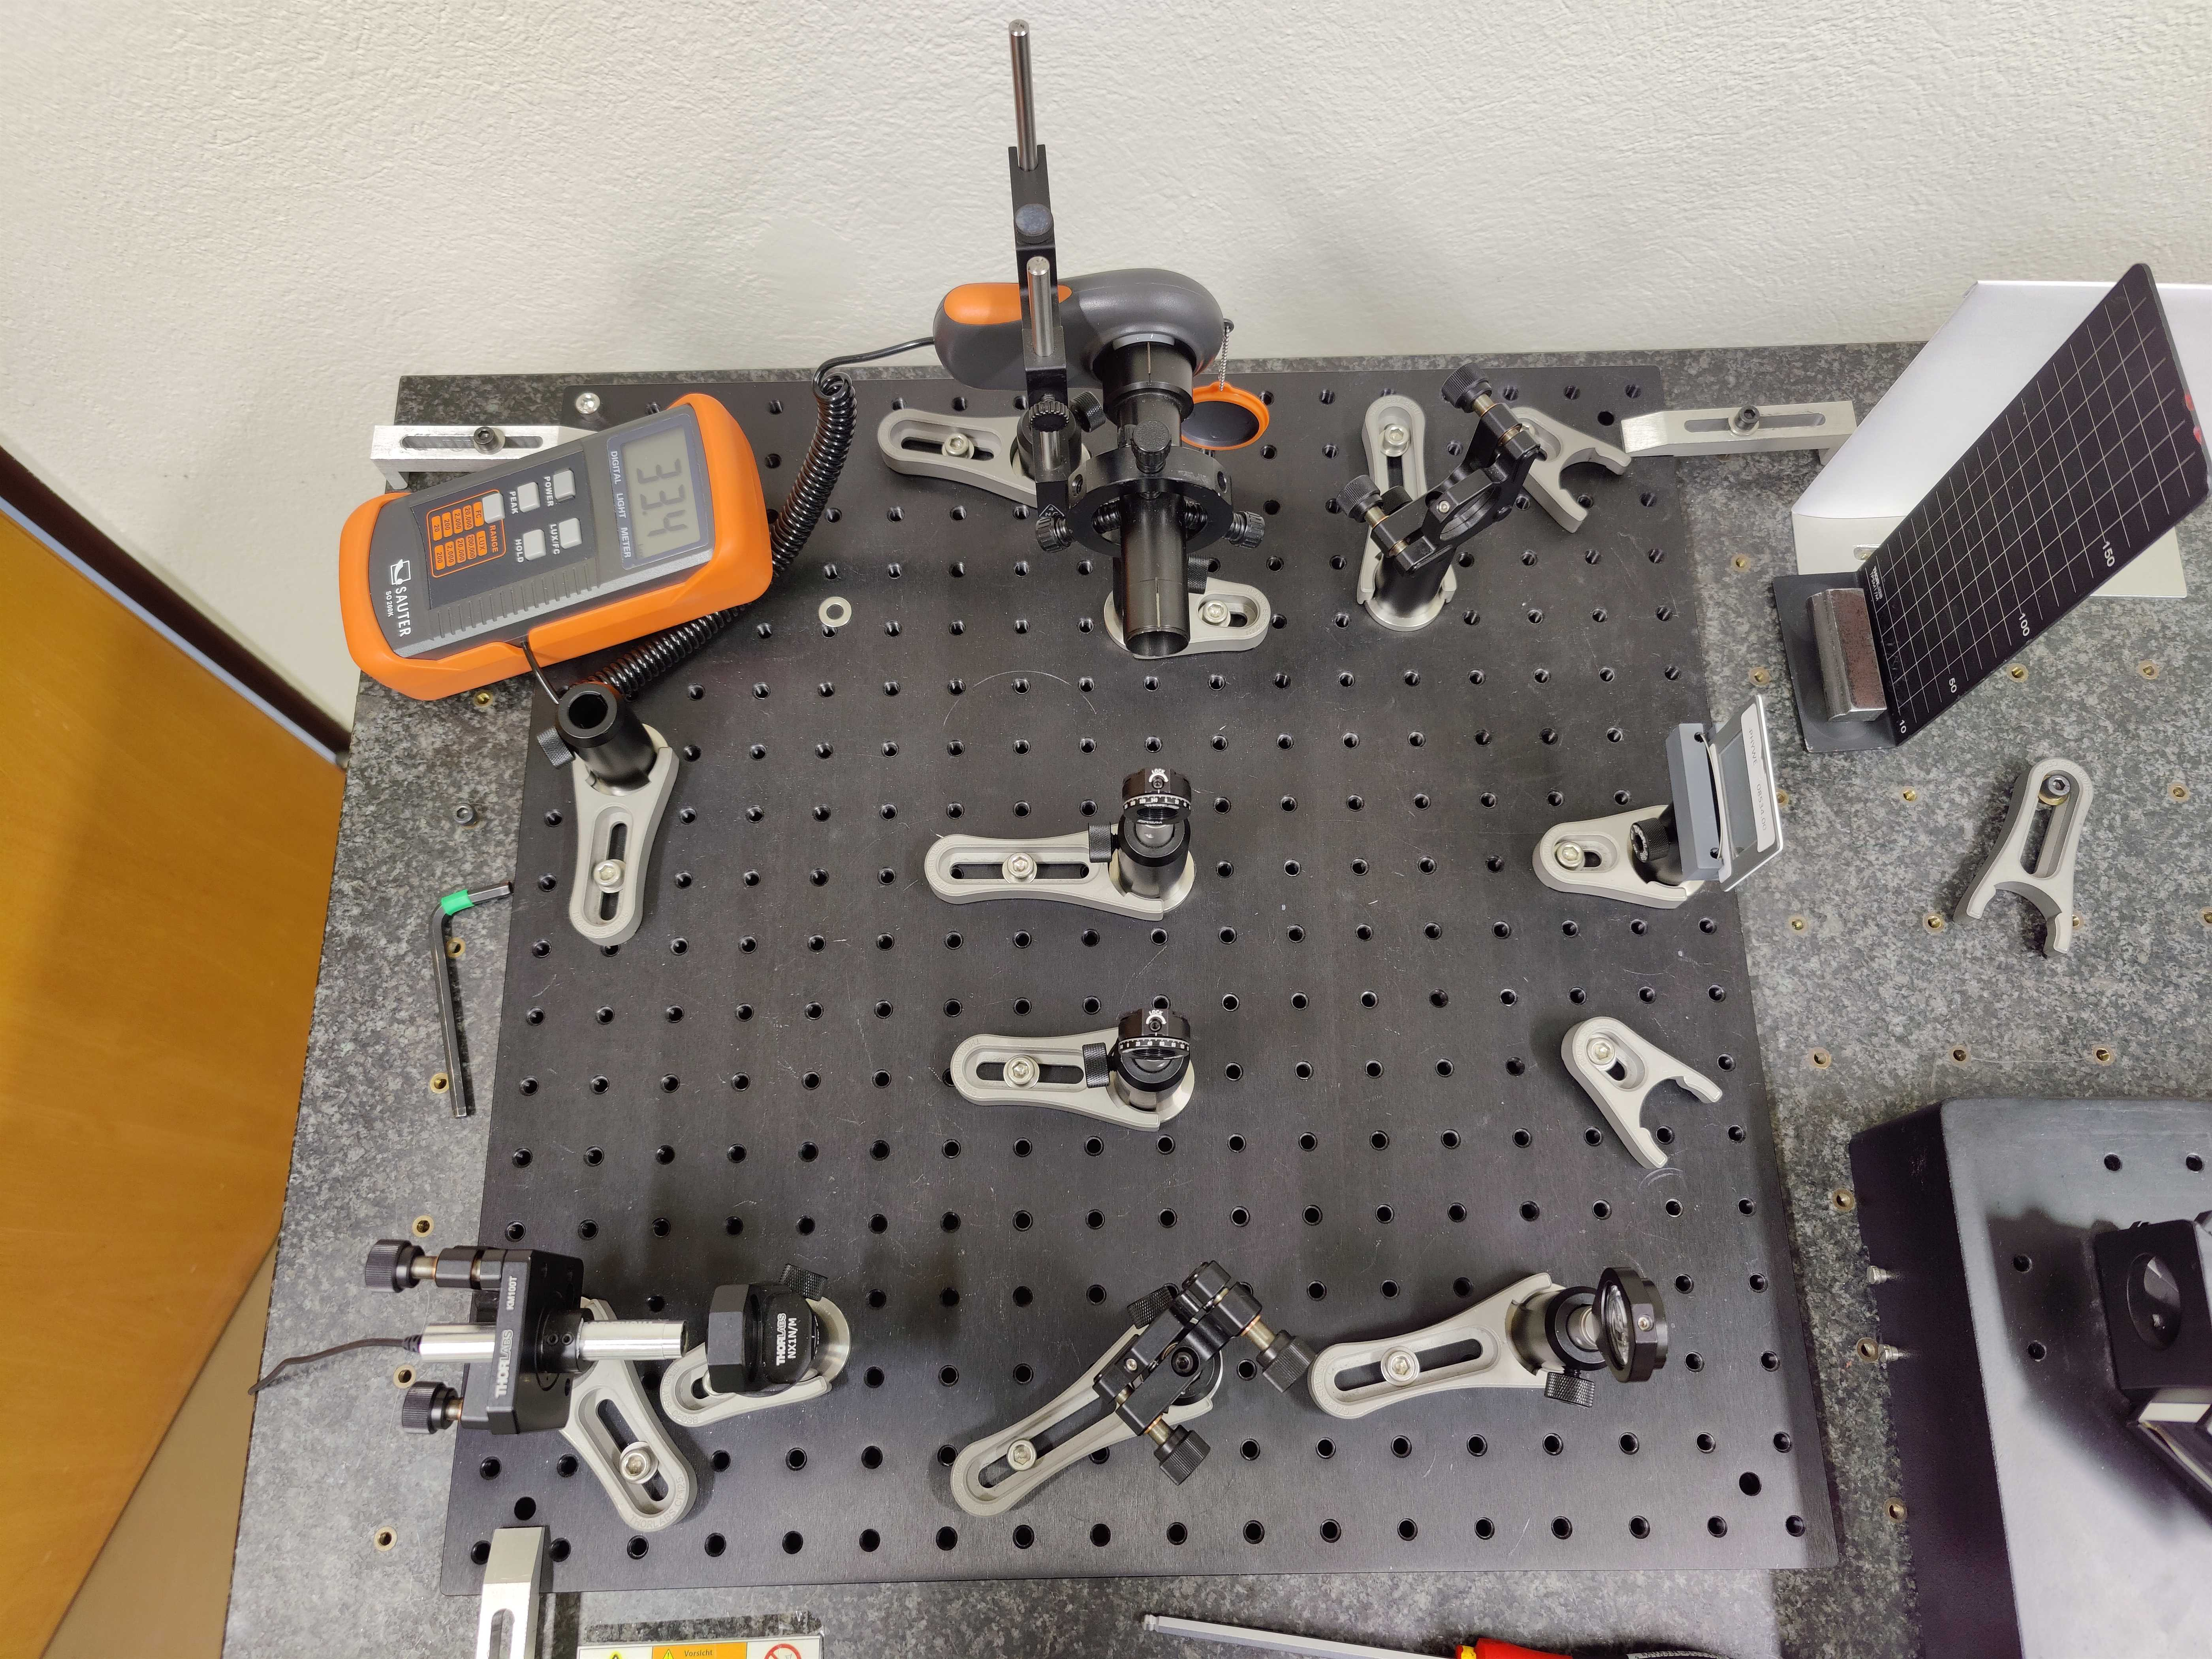
\includegraphics[width=0.7\linewidth]{fig/Aufbau_polarisation.jpg}
        \caption{Aufbau Polarisation}
        \label{fig:aufbau_polarisation}
    \end{samepage}
\end{figure}
\subsection{Michelson Interferometer}
\label{sec:aufbau_michelson}
Nun wird auch der letzte verbleibende Spiegel aus dem Strahlengang des Lasers gegeben und der Laserstrahl trifft so direkt auf das in \autoref{fig:aufbau_michelson} rechts gezeigte Michelson Interferometer. Wie gut in der Abbildung ersichtlich ist, wird der Strahl im Michelson Interferometer in die beiden Arme aufgeteilt. Nach letztlicher Zusammenführung der beiden Strahlen trifft der resultierende Strahl auf den Schirm. 
Zum untersuchen verschiedenen Effekte wird eine Sammel- bzw. Zerstreuungslinse in den Strahlengang zwischen Laser und Michelsoninterfereometer eingebracht. 
\begin{figure}[H]
    \centering
    \begin{samepage}
        \includegraphics[width=0.7\linewidth]{fig/aufbau_michalson.jpg}
        \caption{Aufbau Michelson Interferometer}
        \label{fig:aufbau_michelson}
    \end{samepage}
\end{figure}


\section{Versuchsdurchführung}
\label{sec:durchfuehrung}
Vor jedem Teilversuch wird nochmals überprüft, ob sich ein sinnvoller optischer Weg ergibt und der Laser nicht unkontrolliert oder ungewollt in nicht beabsichtige Richtungen abgelenkt wird. Weiters wird stets darauf geachtet, dass man nicht mit Gegenständen welche \enquote{unkontrolliert} reflektieren (z.B. Ring, Schraubenzieher) in den Strahlengang kommt. 
\subsection{Young'scher Doppelspalt}
\label{sec:durchfuehrung_doppelspalt}
Der Versuch wird gemäß der Beschreibung in \autoref{sec:aufbau_doppelspalte} aufgebaut und die in \autoref{tab:doppelspalt_abmessungen} angeführten Doppelspalte werden der Reihe nach vom Laser durchstrahlt. Der $l_\text{Schirm}$ = \SI{2520(5)}{\milli\meter} entfernte Schirm - ein karriertes A4-Blatt an der Wand - wird nun vom sich ergebendem Interferenzmuster beleuchtet. 

Es ergeben sich für die 4 Doppelspalte folgende Bilder in den Abbildungen \ref{fig:DS_1_interferenzmuster} bis \ref{fig:DS_2_interferenzmuster}. 
\begin{figure}[H]
    \centering
    \begin{samepage}
        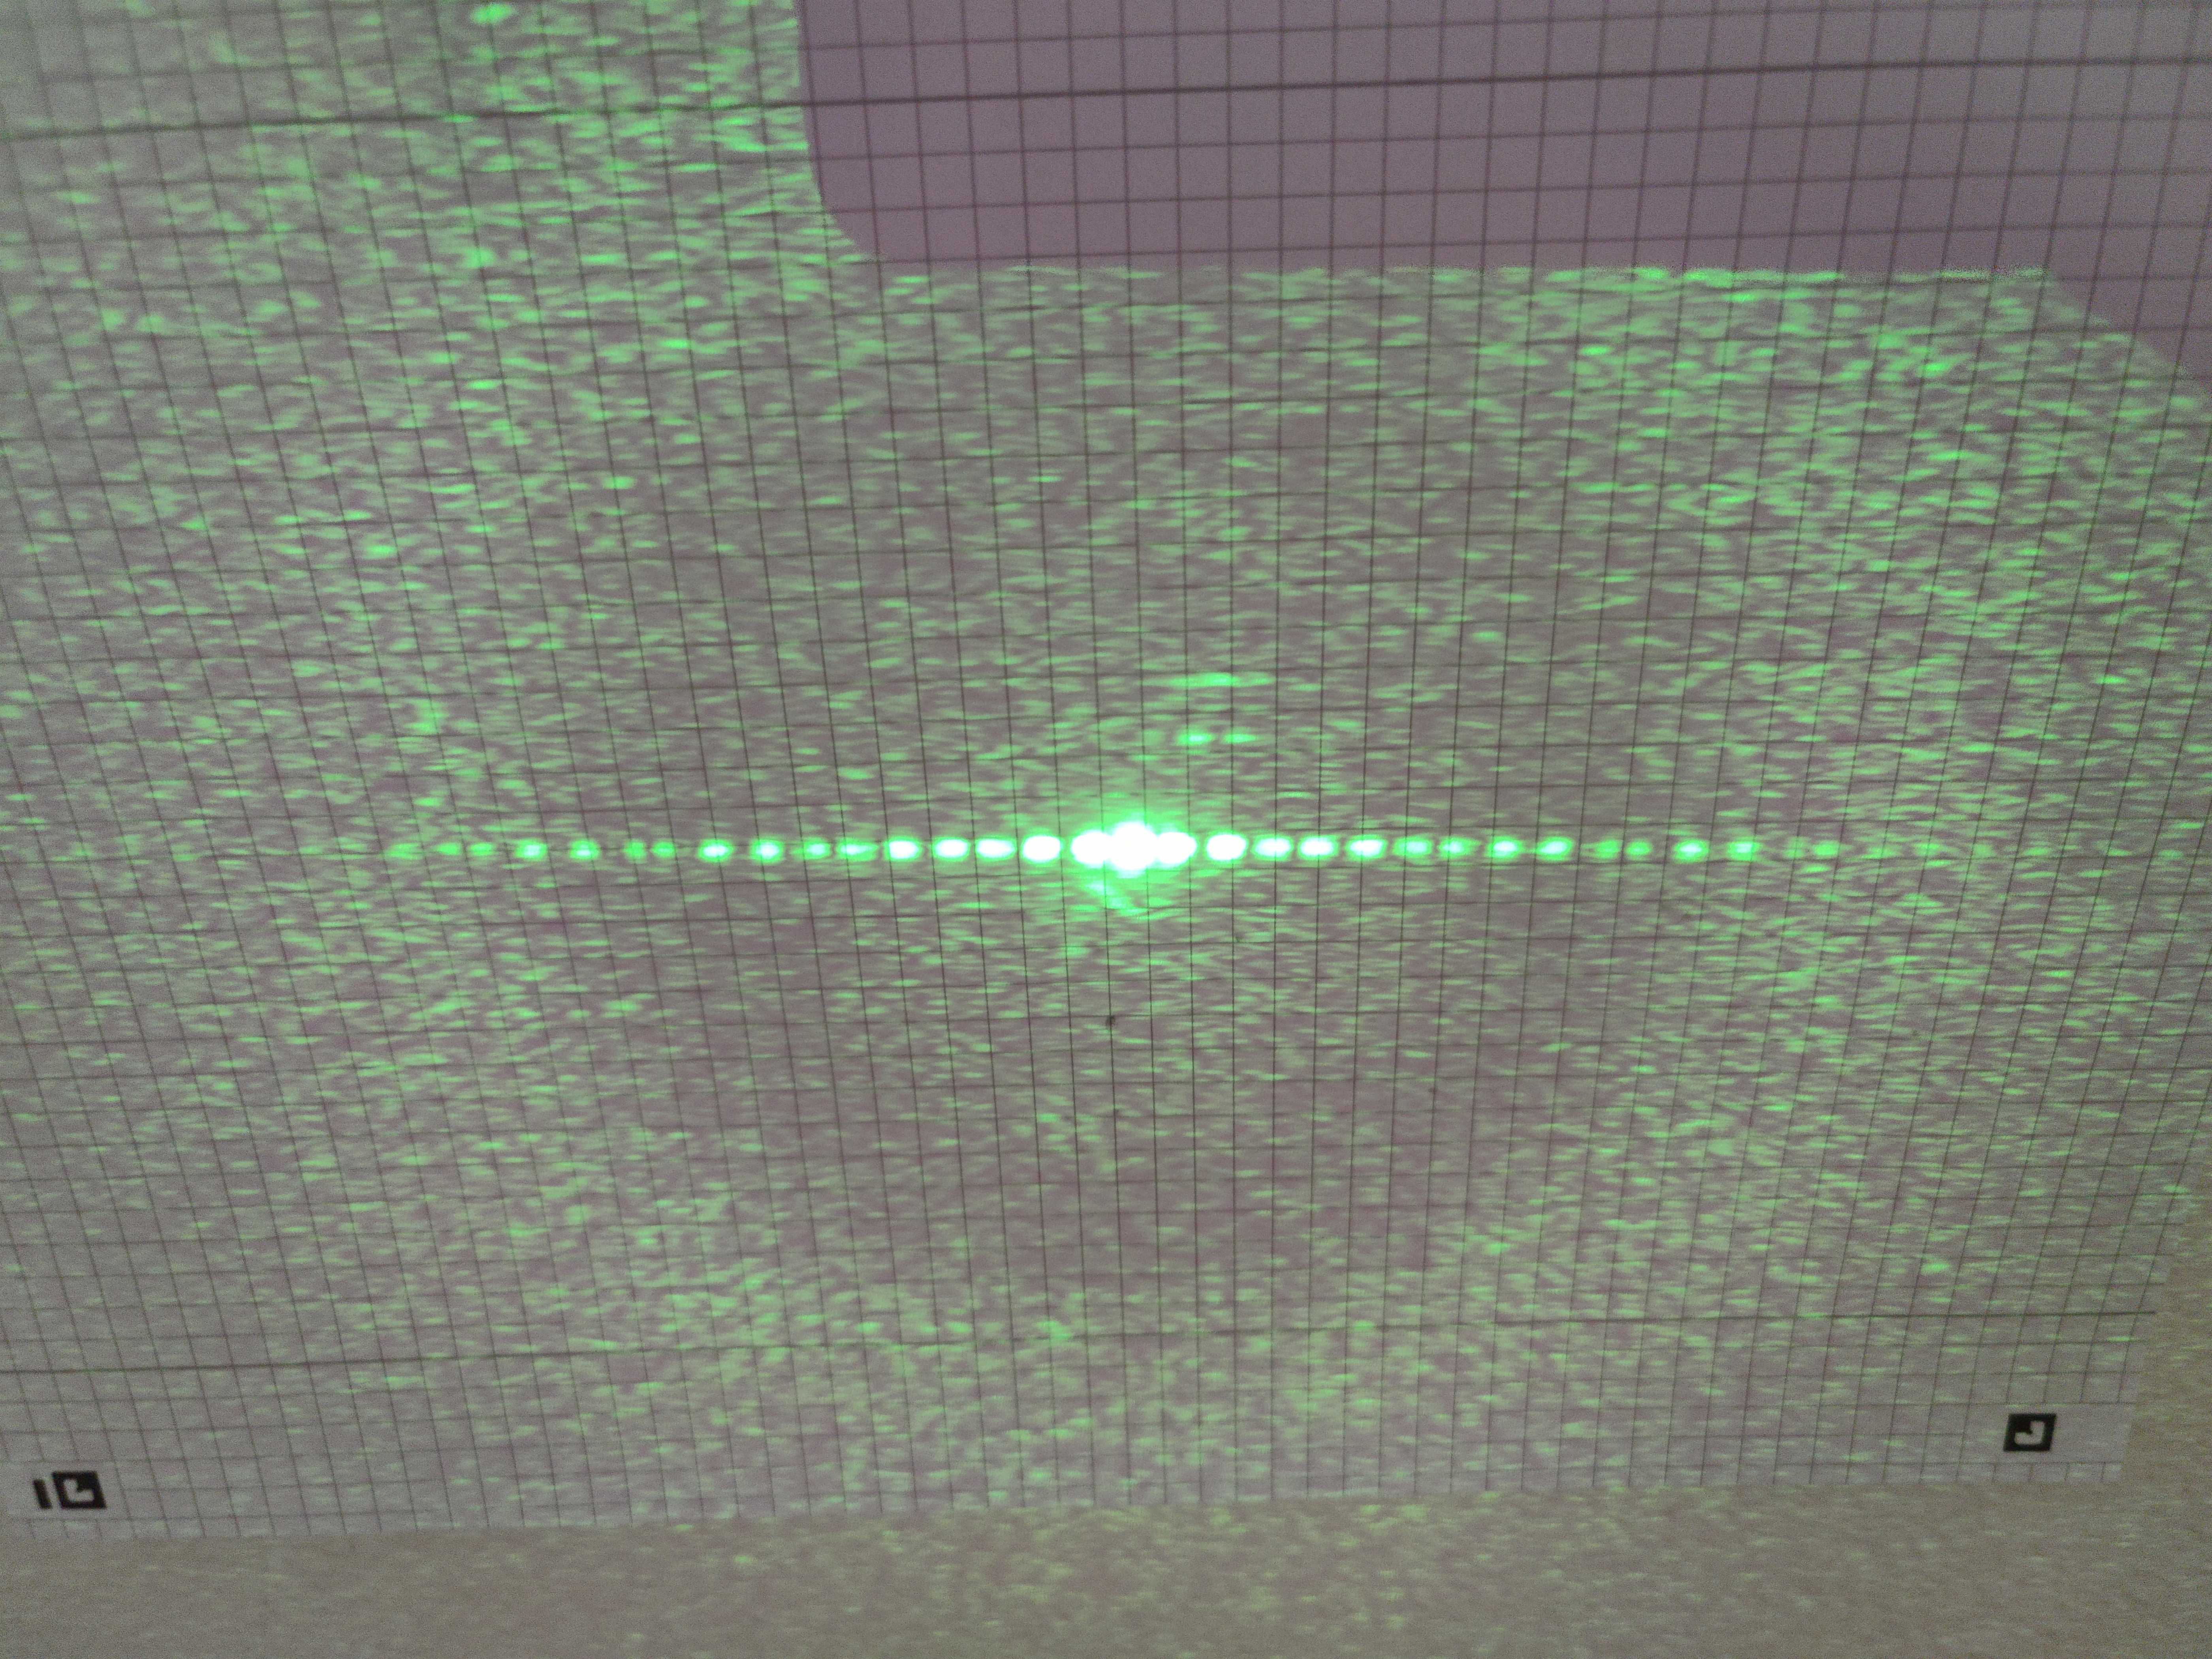
\includegraphics[width=0.7\linewidth]{fig/DS1_0_20_25.jpg}
        \caption{Interferenzmuster des Doppelspalts $i = 1$}
        \label{fig:DS_1_interferenzmuster}
    \end{samepage}
\end{figure}
\begin{figure}[H]
    \centering
    \begin{samepage}
        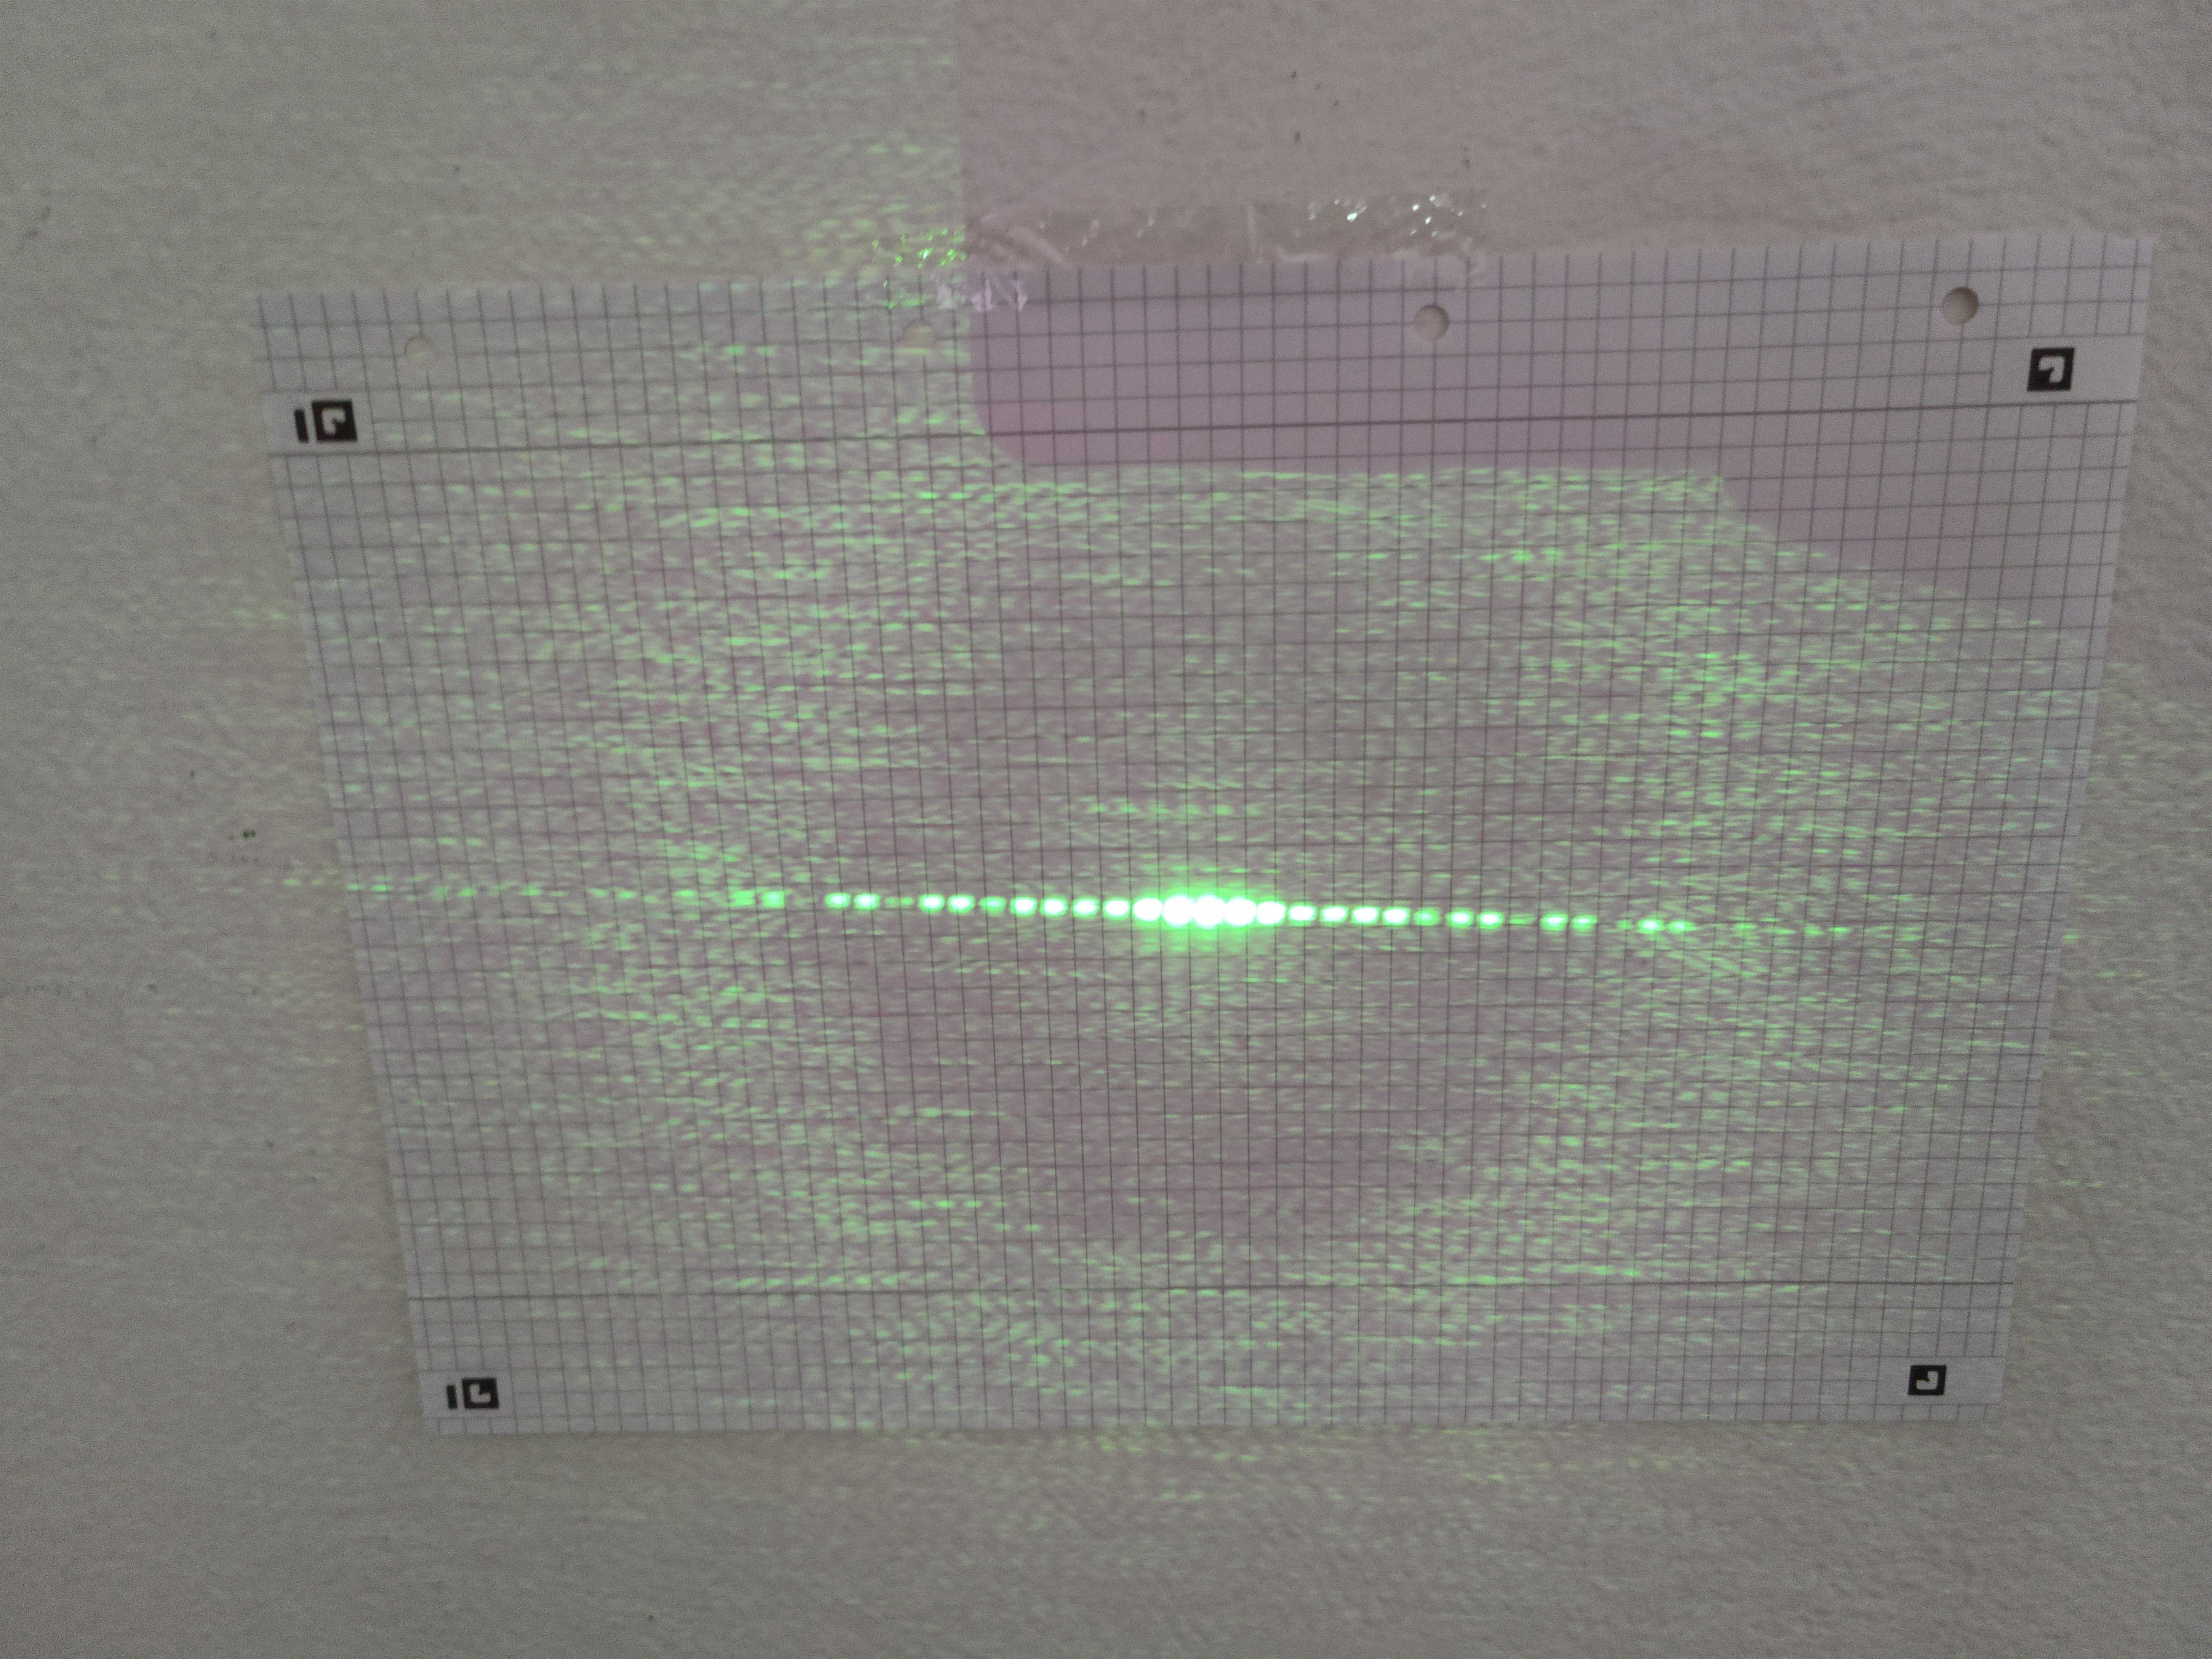
\includegraphics[width=0.7\linewidth]{fig/DS2_0_10_25.jpg}
        \caption{Interferenzmuster des Doppelspalts $i = 2$}
        \label{fig:DS_2_interferenzmuster}
    \end{samepage}
\end{figure}
\begin{figure}[H]
    \centering
    \begin{samepage}
        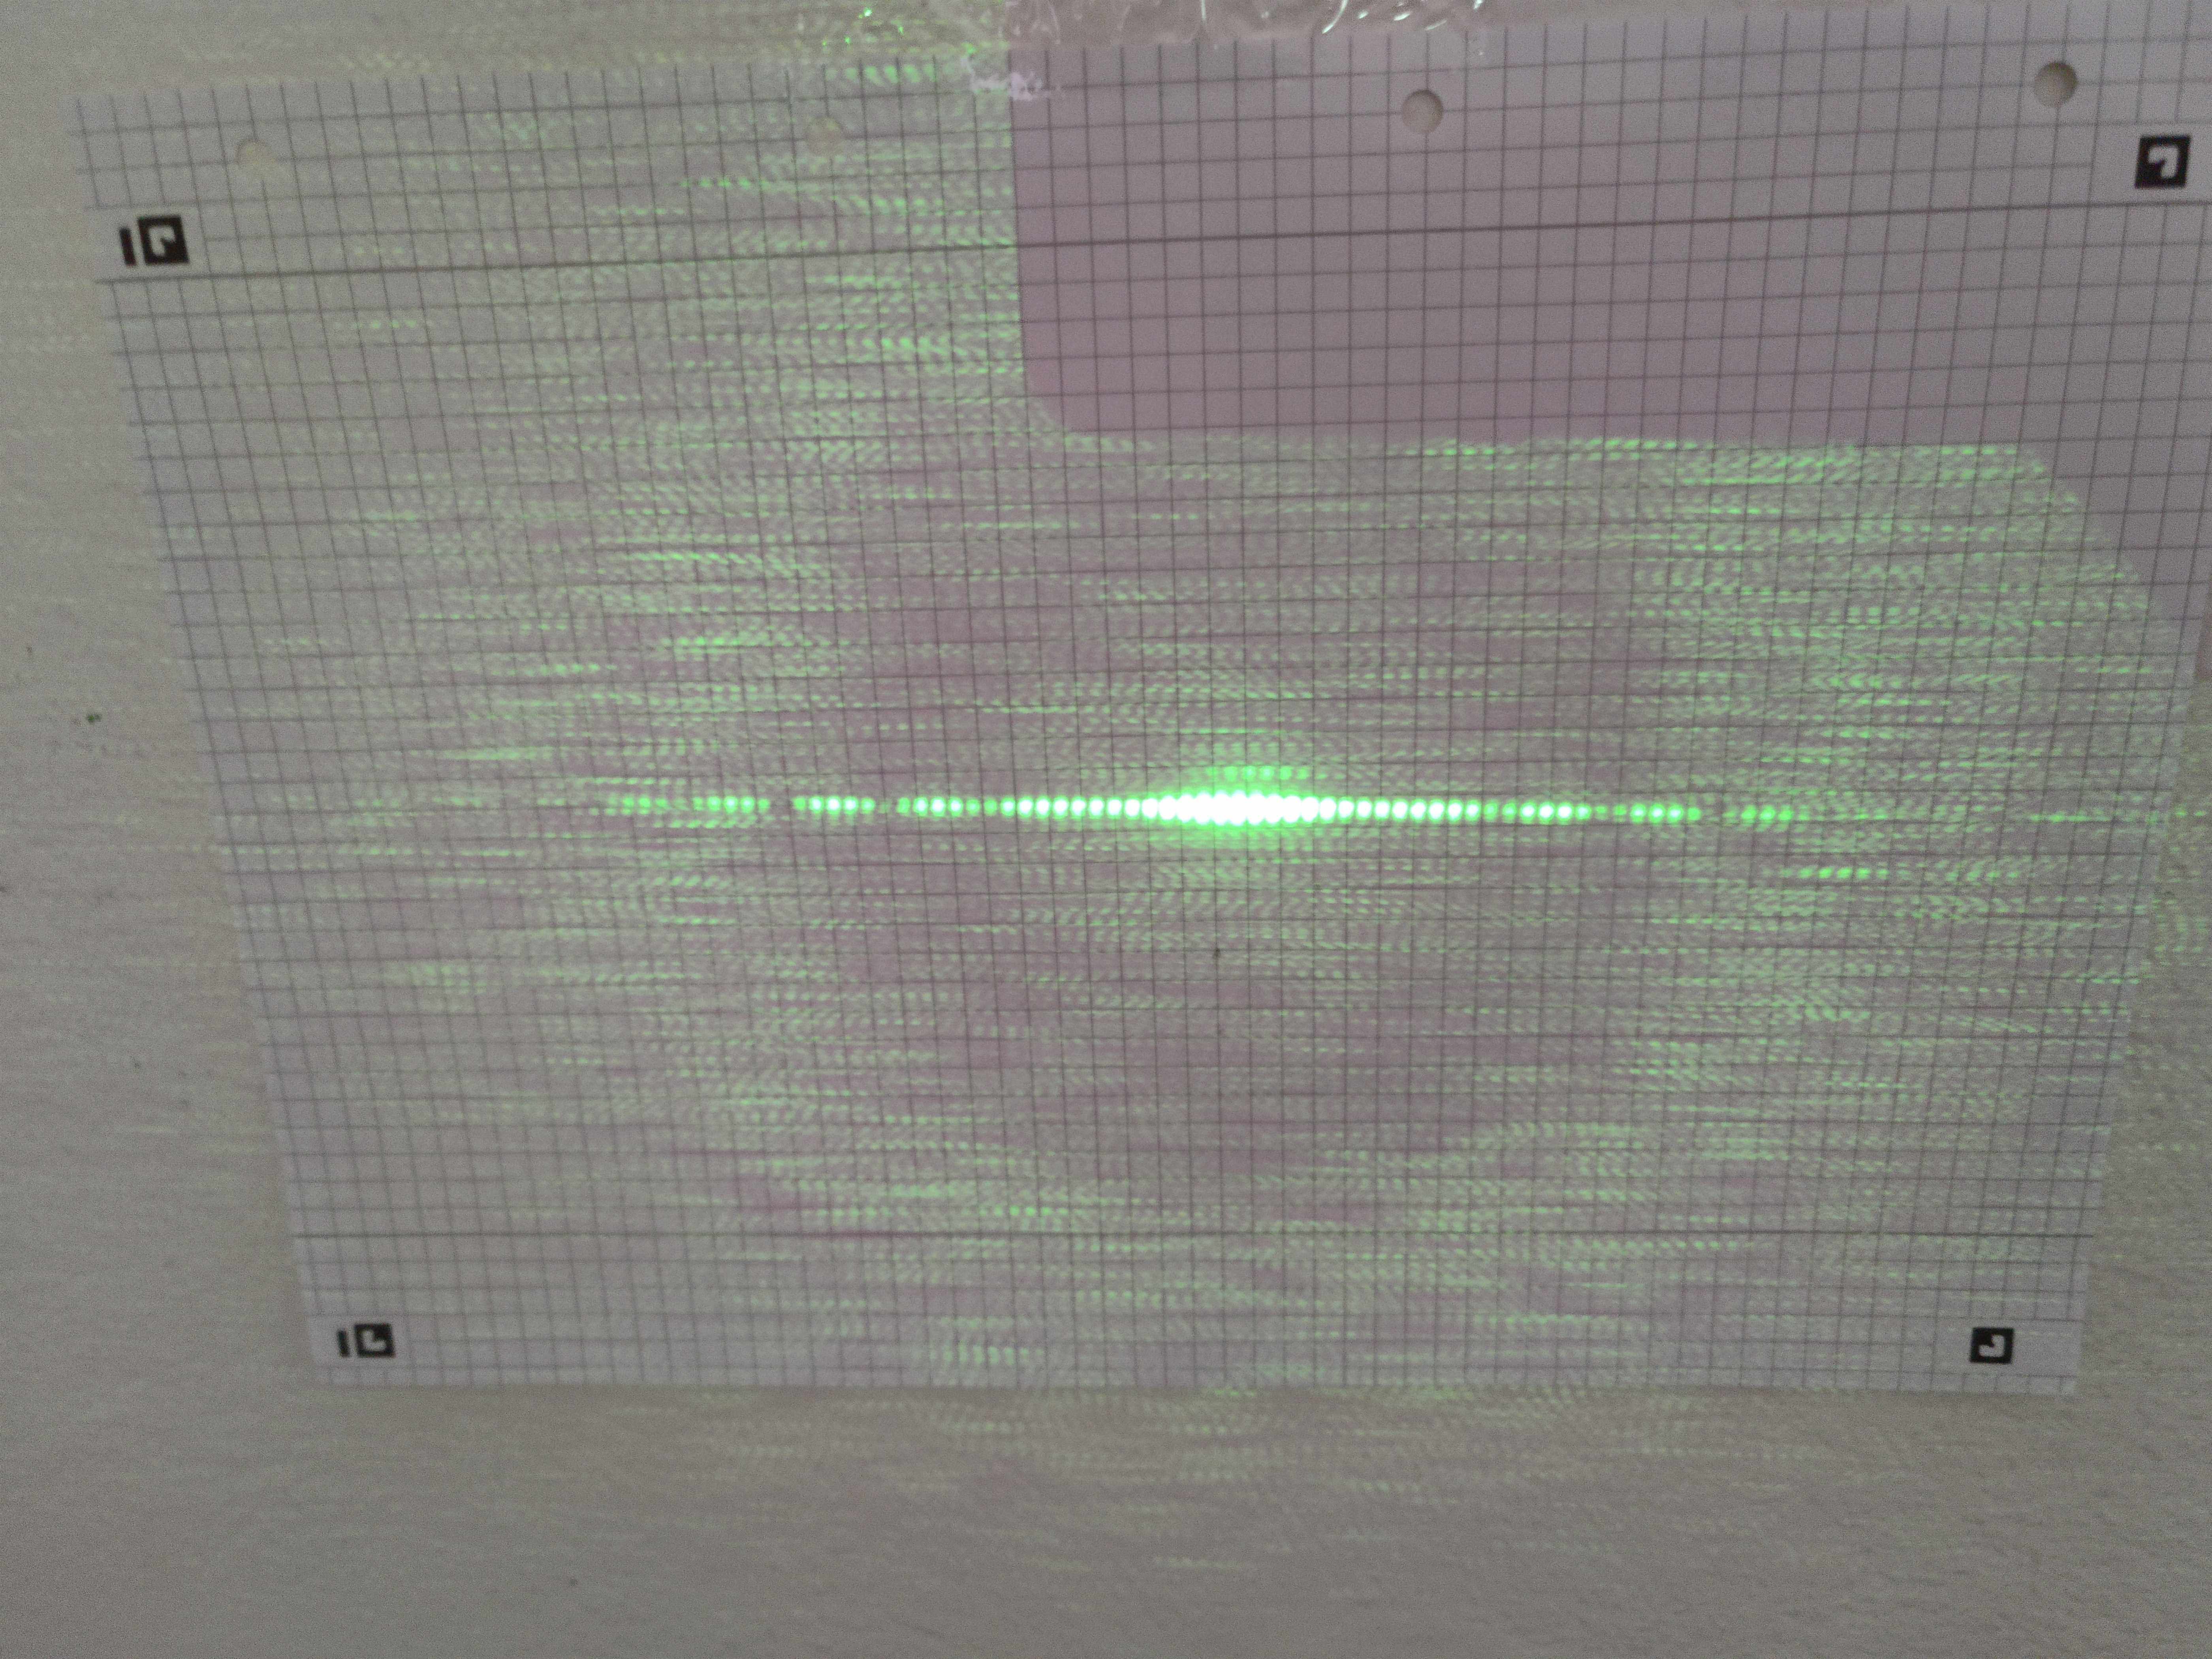
\includegraphics[width=0.7\linewidth]{fig/DS3_0_10_5.jpg}
        \caption{Interferenzmuster des Doppelspalts $i = 3$}
        \label{fig:DS_3_interferenzmuster}
    \end{samepage}
\end{figure}
\begin{figure}[H]
    \centering
    \begin{samepage}
        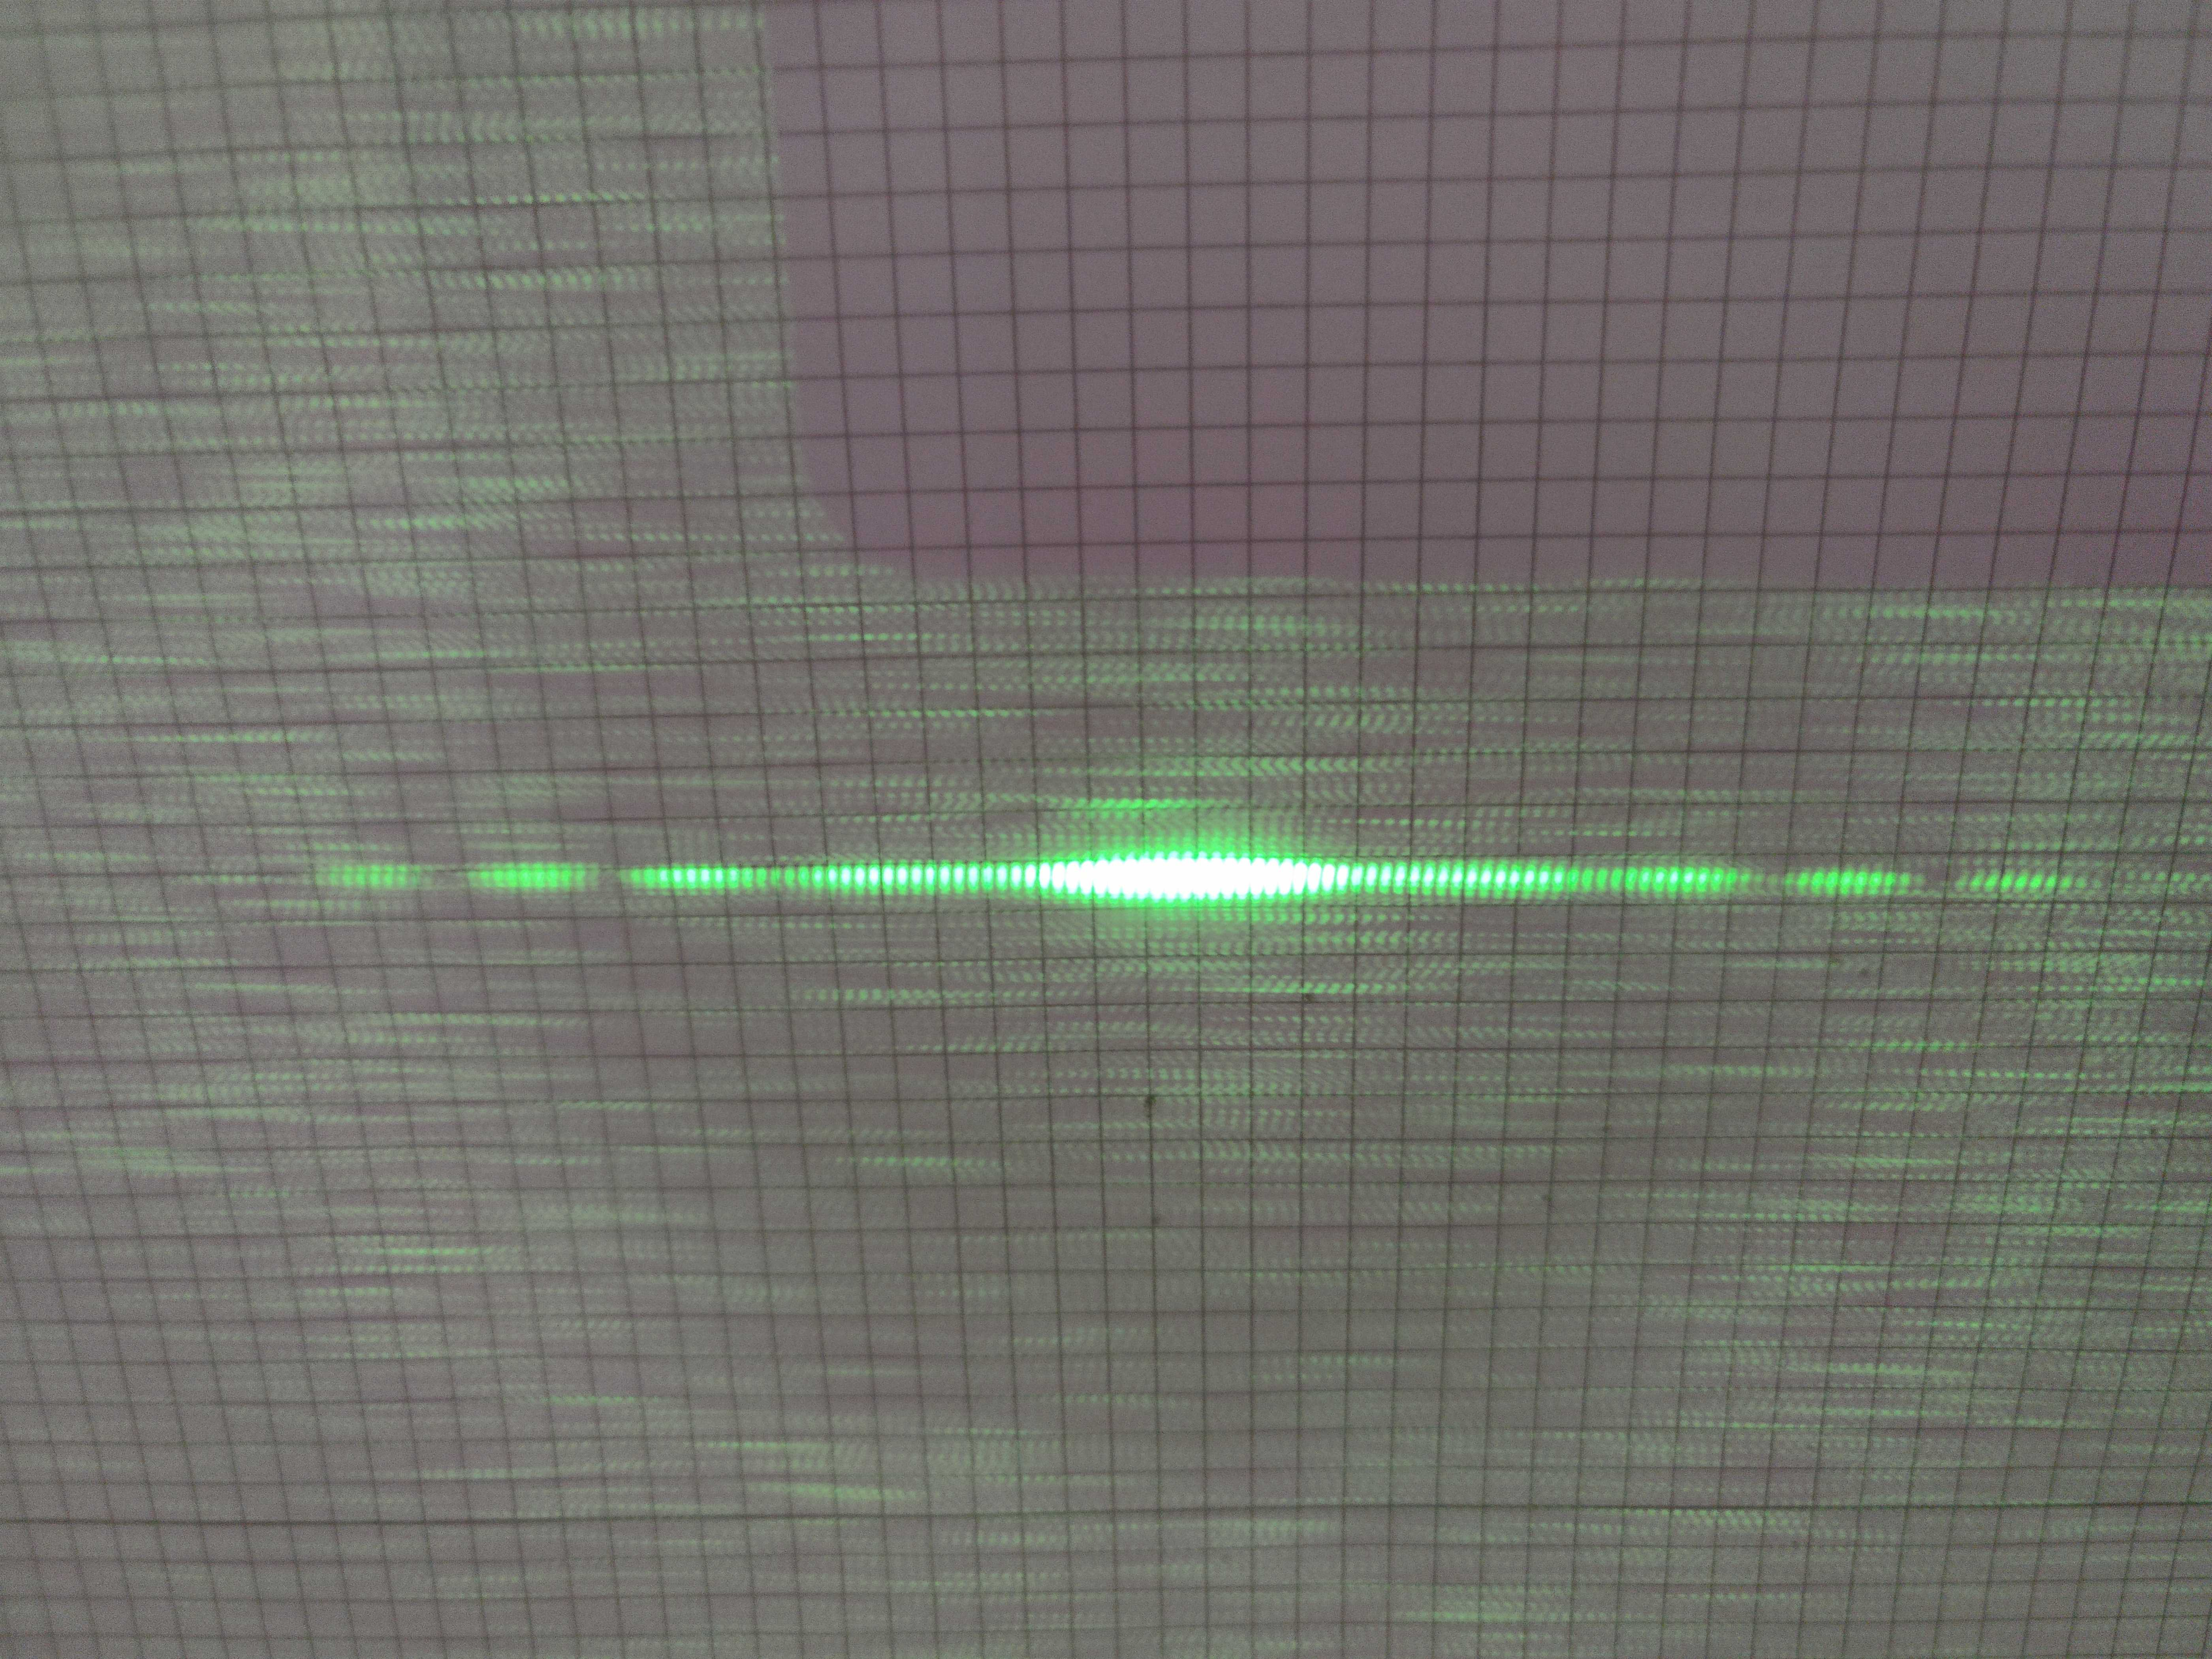
\includegraphics[width=0.7\linewidth]{fig/DS4_0_11.jpg}
        \caption{Interferenzmuster des Doppelspalts $i = 4$}
        \label{fig:DS_4_interferenzmuster}
    \end{samepage}
\end{figure}
Neben der fotografischen Dokumentation werden auch die Abstände der Maxima mittels Lineal vermessen. Die Messungen ergeben die in \autoref{tab:messwerte_doppelspalten} angeführten Werte.

%? Auf meinem laptop geht glaub i tabularray ned gescheit aber vermultich is es nur ein user error :D
% \begin{table}[H]
%     \centering
%     \begin{samepage}
%         \caption[Messwerte Doppelspalten]{Messwerte der Doppelspalten\\Unsicherheit der Messung: $\Delta l_i$ = \SI{0.5}{\milli\meter}
%         \label{tab:messwerte_doppelspalten}
%         \begin{tblr}{colspec={cS[table-format=2.1] S[table-format=2.1] S[table-format=2.1] S[table-format=2.1]}}
%             {{{$i$}}} & {{{$l_1$ / \unit{\milli\meter}}}} & {{{$l_2$ / \unit{\milli\meter}}}} & {{{$l_3$ / \unit{\milli\meter}}}} {{{&$l_4$ / \unit{\milli\meter}}}}\\
%             0 & 0.0 & 0.0 & 0.0 & 0.0\\
%             1 & 5.0 & 5.0 & 2.5 & 1.5\\
%             2 & 11.0& 11.0& 8.0 & 2.5\\
%             3 & 16.0& 16.0& 10.5& 4.0\\
%             4 & 21.0& 22.0& 13.0& 5.5\\
%             5 & 27.0& 27.0& 16.0& 6.5\\
%             6 & 33.0& 32.0& 18.5& 8.0\\
%             7 & 38.0& 38.0& 21.0& 9.5\\
%             8 & 43.0& 43.0& 24.0& 10.5\\
%             9 & 49.0& 48.0& 26.5& 12.0\\
%             10& 55.0& 54.0& 29.0& 13.5\\
%             11& 58.0& -   & -   & 15.0\\
%         \end{tblr}
%     \end{samepage}
% \end{table}

Die obige Messung wird nun in analoger Weise nochmals mit dem Gitter durchgeführt. Die Messungen ergeben die in \autoref{tab:messwerte_gitter} angeführten Werte. Dabei bleibt der Abstand zum Schirm $l_\text{Schirm}$ = \SI{2520(5)}{\milli\meter} konstant.
% \begin{table}[H]
%     \centering
%     \begin{samepage}
%         \caption[Messwerte Gitter]{Messwerte des Gitters\\Unsicherheit der Messung: $\Delta l_i$ = \SI{0.5}{\milli\meter}
%         \label{tab:messwerte_gitter}
%         \begin{tblr}{colspec={cS[table-format=3.1]}}
%             {{{$i$}}} & {{{$l_1$ / \unit{\milli\meter}}}} \\
%             0  & 0.0\\
%             1  & 11.0\\
%             2  & 21.5\\
%             3  & 32.5\\
%             4  & 43.0\\
%             5  & 53.5\\
%             6  & 64.5\\
%             7  & 75.0\\
%             8  & 86.0\\
%             9  & 97.0\\
%             10 & 108.0\\
%             11 & 118.0\\
%             12 & 128.0\\
%             13 & 139.0\\
%             14 & 151.0\\
%         \end{tblr}
%     \end{samepage}
% \end{table}

\subsection{Shearing Interferometer}
\label{sec:durchfuehrung_shearing}
Der Aufbau erfolgt gemäß \autoref{sec:aufbau_shearing} und die der Laser wird mittels Spiegel wie beschrieben auf das Interferometer gelenkt. 

Aus dem am Shearing Interferometer entstandenem Interferenzmuster wird werden nun die drei Größen: $l$ Versatz in laterale Richtung, $\Theta$ Winkelversatz zur einfallenden Ebene und der Streifenabstand $d$ bestimmt. Die Messungen ergeben sich zu: 
%!Natürlich komplett frei erfunden
\begin{itemize}
    \item $l$ = \SI{8.0(5)}{\milli\meter}
    \item $\Theta$ = \SI{-19(3)}{\degree}
    \item $d$ = \SI{4.0(5)}{\milli\meter}
\end{itemize}
\subsection{Polarisation}
\label{sec:durchfuehrung_polarisation}
Der Strahl wird für den ersten Unterpunkt dieses Versuchs durch zwei Polarisationsfilter geführt. Für den ersten der beiden Filter wurde \SI{70}{\degree} als Ausgangswinkel gewählt, der zweite wird im folgenden Versuch einmal um \SI{360}{\degree} gedreht, wobei die Ausgangsstellung hier so gewählt wird, dass zuerst die höchste Lichtintensität am Messgerät abgelesen werden kann. So stehen die Polarisationsfilter gleich; Dies ist bei \SI{330}{\degree} des zweiten Filters der Fall. 
Die Messung wurde zweimal durchgeführt und die gemessenen Werte des Lichtintensitätsmesser sind in \autoref{tab:messwerte_polarisation} angeführt.
% \begin{table}[H] 
%     \centering
%     \begin{samepage}
%         \caption[Messwerte Polarisation]{Messwerte nach Durchgang durch zwei Polarisationsfilter \\Winkel des ersten Filters: \SI{70}{\degree}, Winkel des zweiten Filters $\alpha$ mit $\Delta \alpha$ = \SI{3}{\degree}, Intensität $I$ }
%         \label{tab:messwerte_polarisation}
%         \begin{tblr}{colspec={S[table-format=3.0]S[table-format=4.0]S[table-format=4.0]}}
%             {{{$\alpha$}}} & {{{$I_1$ / \unit{\lux}}}}& {{{$I_2$ / \unit{\lux}}}} & {{{$\Delta I_1$ / \unit{\lux}}}} & {{{$\Delta I_2$ / \unit{\lux}}}} \\
% 330.0   & 1022.0        & 1074.0        & 40.66         & 42.22 \\
% 340.0   & 999.0         & 1050.0        & 39.97         & 41.5  \\
% 350.0   & 911.0         & 966.0         & 37.33         & 38.98 \\
% 0.0     & 781.0         & 820.0         & 33.43         & 34.6  \\
% 10.0    & 617.0         & 643.0         & 28.51         & 29.29 \\
% 20.0    & 444.0         & 456.0         & 23.32         & 23.68 \\
% 30.0    & 279.0         & 285.0         & 18.37         & 18.55 \\
% 40.0    & 132.0         & 142.0         & 13.96         & 14.26 \\
% 50.0    & 37.0  & 38.0  & 11.11         & 11.14 \\
% 60.0    & 0.0   & 0.0   & 10.0  & 10.0  \\
% 70.0    & 24.0  & 26.0  & 10.72         & 10.78 \\
% 80.0    & 108.0         & 110.0         & 13.24         & 13.3  \\
% 90.0    & 236.0         & 252.0         & 17.08         & 17.56 \\
% 100.0   & 397.0         & 412.0         & 21.91         & 22.36 \\
% 110.0   & 578.0         & 603.0         & 27.34         & 28.09 \\
% 120.0   & 756.0         & 793.0         & 32.68         & 33.79 \\
% 130.0   & 896.0         & 943.0         & 36.88         & 38.29 \\
% 140.0   & 1000.0        & 1046.0        & 40.0  & 41.38 \\
% 150.0   & 1047.0        & 1097.0        & 41.41         & 42.91 \\
% 160.0   & 1028.0        & 1074.0        & 40.84         & 42.22 \\
% 170.0   & 950.0         & 993.0         & 38.5  & 39.79 \\
% 180.0   & 816.0         & 847.0         & 34.48         & 35.41 \\
% 190.0   & 653.0         & 679.0         & 29.59         & 30.37 \\
% 200.0   & 471.0         & 490.0         & 24.13         & 24.7  \\
% 210.0   & 288.0         & 304.0         & 18.64         & 19.12 \\
% 220.0   & 150.0         & 150.0         & 14.5  & 14.5  \\
% 230.0   & 38.0  & 43.0  & 11.14         & 11.29 \\
% 240.0   & 0.0   & 0.0   & 10.0  & 10.0  \\
% 250.0   & 25.0  & 24.0  & 10.75         & 10.72 \\
% 260.0   & 114.0         & 121.0         & 13.42         & 13.63 \\
% 270.0   & 257.0         & 263.0         & 17.71         & 17.89 \\
% 280.0   & 421.0         & 440.0         & 22.63         & 23.2  \\
% 290.0   & 607.0         & 635.0         & 28.21         & 29.05 \\
% 300.0   & 747.0         & 819.0         & 32.41         & 34.57 \\
% 310.0   & 927.0         & 971.0         & 37.81         & 39.13 \\
% 320.0   & 1029.0        & 1070.0        & 40.87         & 42.1  \\
% 330.0   & 1067.0        & 1109.0        & 42.01         & 43.27 \\
%         \end{tblr}
%     \end{samepage}
% \end{table}


\subsection{Michelson Interferometer}
\label{sec:durchfuehrung_michelson}



\section{Auswertung}
\label{sec:auswertung}

% \setcapindent{0pt}
% \begin{figure}[H]
%     \centering
%     \begin{minipage}[t]{0.45\linewidth}
%         \centering
%         \includegraphics[width=\linewidth]{plots/stern_allgemein.png}
%         \caption[Zeigerdiagramm allgemeine Sternschaltung]{Zeigerdiagramm allgemeine Sternschaltung, Strom $I_{xx}$ in \si{\centi\ampere} und Spannung $U_{xx}$ in \si{\volt}}
%         \label{fig:stern_asym_allg_zeigerdiagramm}
%     \end{minipage}%
%     \hspace*{\fill}
%     \begin{minipage}[t]{0.45\linewidth}
%         \centering
%         \includegraphics[width=\linewidth]{plots/stern_allgemein_tausch.png}
%         \caption[Zeigerdiagramm allgemeine Sternschaltung mit vertauschten Außenleitern ($\text{L2} \leftrightarrow \text{L3}$)]{Zeigerdiagramm allgemeine Sternschaltung mit vertauschten Außenleitern ($\text{L2} \leftrightarrow \text{L3}$), Strom $I_{xx}$ in \si{\centi\ampere} und Spannung $U_{xx}$ in \si{\volt}}
%         \label{fig:stern_asym_allg_tausch_zeigerdiagramm}
%     \end{minipage}
% \end{figure}
% \setcaphanging




\section{Diskussion}
\label{sec:diskussion}


\section{Zusammenfassung}
\label{sec:zusammenfassung}


\clearpage
% Literaturverzeichnis
\printbibliography

% Abbildungsverzeichnis
\listoffigures

% Tabellenverzeichnis
\listoftables


\end{document}